% 
\documentclass[cic,tc]{iiufrgs}

% Use unicode
\usepackage[utf8]{inputenc}   % pacote para acentuação
\usepackage{amsmath}

% Necessário para incluir figuras
\usepackage{graphicx}         % pacote para importar figuras

\usepackage{times}            % pacote para usar fonte Adobe Times
% \usepackage{palatino}
% \usepackage{mathptmx}       % p/ usar fonte Adobe Times nas fórmulas

\usepackage[alf,abnt-emphasize=bf]{abntex2cite}	% pacote para usar citações abnt

\usepackage{array}
% 
% Informações gerais
% 
\title{Implementação e Avaliação de um Mecanismo de Detecção de Ameaças em uma Ferramenta Smart Grid}

\author{Eitelvein}{Luiza dos Santos}

\advisor[Prof.~Dr.]{Schaeffer-Filho}{Alberto Egon}

% a data deve ser a da defesa; se nao especificada, são gerados
% mes e ano correntes
% \date{dezembro}{2015}

 \location{Porto Alegre}{RS}

% itens individuais da nominata podem ser redefinidos com os comandos
% abaixo:
% \renewcommand{\nominataReit}{Prof\textsuperscript{a}.~Wrana Maria Panizzi}
% \renewcommand{\nominataReitname}{Reitora}
% \renewcommand{\nominataPRE}{Prof.~Jos{\'e} Carlos Ferraz Hennemann}
% \renewcommand{\nominataPREname}{Pr{\'o}-Reitor de Ensino}
% \renewcommand{\nominataPRAPG}{Prof\textsuperscript{a}.~Joc{\'e}lia Grazia}
% \renewcommand{\nominataPRAPGname}{Pr{\'o}-Reitora Adjunta de P{\'o}s-Gradua{\c{c}}{\~a}o}
% \renewcommand{\nominataDir}{Prof.~Philippe Olivier Alexandre Navaux}
% \renewcommand{\nominataDirname}{Diretor do Instituto de Inform{\'a}tica}
% \renewcommand{\nominataCoord}{Prof.~Carlos Alberto Heuser}
% \renewcommand{\nominataCoordname}{Coordenador do PPGC}
% \renewcommand{\nominataBibchefe}{Beatriz Regina Bastos Haro}
% \renewcommand{\nominataBibchefename}{Bibliotec{\'a}ria-chefe do Instituto de Inform{\'a}tica}
% \renewcommand{\nominataChefeINA}{Prof.~Jos{\'e} Valdeni de Lima}
% \renewcommand{\nominataChefeINAname}{Chefe do \deptINA}
% \renewcommand{\nominataChefeINT}{Prof.~Leila Ribeiro}
% \renewcommand{\nominataChefeINTname}{Chefe do \deptINT}

% 
% palavras-chave
% iniciar todas com letras minúsculas, exceto no caso de abreviaturas
% 
\keyword{smart grid}


%\settowidth{\seclen}{1.10~}

% 
% inicio do documento
% 
\begin{document}

% folha de rosto
% às vezes é necessário redefinir algum comando logo antes de produzir
% a folha de rosto:
% \renewcommand{\coordname}{Coordenadora do Curso}
\maketitle

% dedicatoria
% \clearpage
% \begin{flushright}
%     \mbox{}\vfill
%     {\sffamily\itshape
%       ``If I have seen farther than others,\\
%       it is because I stood on the shoulders of giants.''\\}
%     --- \textsc{Sir~Isaac Newton}
% \end{flushright}

% agradecimentos
%\chapter*{Agradecimentos}
%Agradeço ao \LaTeX\ por não ter vírus de macro\ldots



% resumo na língua do documento
\begin{abstract}
    Resumo em português.
\end{abstract}

% resumo na outra língua
% como parametros devem ser passados o titulo e as palavras-chave
% na outra língua, separadas por vírgulas
\begin{englishabstract}{Implementation and Evaluation of a Threat Detection Mechanism in a Smart Grid Tool}{Smart Grid}
    Abstract in English.
\end{englishabstract}

% lista de figuras
\listoffigures

% lista de tabelas
\listoftables

% lista de abreviaturas e siglas
% o parametro deve ser a abreviatura mais longa
\begin{listofabbrv}{SCADA}
    \item[AMI]   Advanced Monitoring Infrastructure
    \item[ABD]   Anomaly Based Detection
    \item[ADU]   Application Data Unit
    \item[DC]    Dispositivo de Campo
    \item[DEI]   Dispositivo Eletrônico Inteligente
    \item[HIDS]  Host Based Intrusion Detection System
    \item[ICT]   Information and Communication Technology
    \item[IDS]   Intrusion Detection System
    \item[IHM]   Interface Homem-Máquina
    \item[IP]    Internet Protocol
    \item[ML]    Machine Learning
    \item[MTU]   Master Terminal Unit
    \item[NIDS]  Network Based Intrusion Detection System
    \item[OCSVM] One-Class Suport Vectors Machine
    \item[PLC]   Programmable Logic Controller
    \item[RTU]   Remote Terminal Unit
    \item[SBD]   Signature Based Detection
    \item[SCADA] Supervisory Control and Data Acquisition
    \item[SCI]   Sistema de Controle Industrial  
	\item[SVM]   Suport Vectors Machine
	\item[TCP]   Transmission Control Protocol
	\item[UDP]   User Datagram Protocol
    
\end{listofabbrv}

% idem para a lista de símbolos
% \begin{listofsymbols}{$\alpha\beta\pi\omega$}
%     \item[$\sum{\frac{a}{b}}$] Somatório do produtório
%     \item[$\alpha\beta\pi\omega$] Fator de inconstância do resultado
% \end{listofsymbols}

% sumario
\tableofcontents

\chapter{Introdução}
\section{Motivação}
\section{Objetivos}
\section{Contribuição}
\section{Estrutura do Trabalho}
\chapter{Fundamentação Teórica}
Neste capítulo, será estabelecida a fundamentação teórica dos tópicos abordados neste trabalho, afim de fornecer o entendimento dos conceitos e tecnologias que serão utilizados e apresentar o estado da arte em que se encontram. A seção \ref{secsg} introduz os smart grids, seu propósito, sua arquitetura e as ameaças que os afetam. Na seção \ref{secmec}, são abordados os mecanismos de segurança utilizados em smart grids. Finalmente, a seção \ref{sectools} apresenta as ferramentas existentes para simulação de ambientes smart grid e sistemas SCADA.

\section{Smart Grids}
\label{secsg}
Smart Grids combinam redes de energia elétrica com estruturas de comunicação, baseadas em Tecnologia de Informação e Comunicação - \emph{Infomation and Communication Technology (ICT)}, que provêm um meio de troca de dados entre os componentes envolvidos no processo de produção, distribuição e consumo de energia. Como suas principais características, podem ser mencionados o fluxo bidirecional de energia elétrica entre produtores e consumidores e a incorporação de uma infraestrutura de comunicação, também bidirecional, que provê uma maior capacidade de automação à rede \cite{2013survey}. Através de recursos e técnicas como monitoramento em tempo real, automação e controle de dispositivos, autoavaliação e autorecuperação, integração com de fontes de energia alternativas e mecanismos de segurança física e cibernética, Smart Grids imbuem a rede elétrica com maior confiabilidade, eficiência e segurança \cite{li2012securing}.

A Seção \ref{subsecmotiv} as motivações para o crescimento do uso de smart grids. Na Seção \ref{subsecarq}, é mostrada a arquitetura dos smart grids. A Seção \ref{subsecthreats} discute as ameaças às quais os smart grids são suscetíveis.

\subsection{Motivação}
\label{subsecmotiv}

A  infraestrutura de comunicação dos Smart Grids incorpora uma grande diversidade de benefícios ao sistema de produção, distribuição e consumo de energia. Dados coletados pela Infraestrutura de Monitoramento Avançada - \emph{Advanced Metering Infrastructure (AMI)} podem ser utilizados para melhorar a eficiência e o desempenho da distribuição de energia, identificando picos de consumo e pontos de desperdício na rede, além de fornecer aos usuários informações detalhadas sobre seu consumo de energia, levando-os a um consumo mais eficiente. Uma maior automação da rede de distribuição leva à diminuição dos custos operacionais, pois seu funcionamento torna-se mais independente da mão de obra envolvida, que, por sua vez, pode executar suas tarefas com mais eficiência. A capacidade de comunicação entre diversas entidades e o fluxo bidirecional de energia possibilitam uma utilização cada vez maior de recursos de energia distribuídos, incentivando o surgimento de fontes de geração de energia renovável, como solar e eólica. Entidades consumidoras podem também ser produtoras de energia, permitindo que microprodutores forneçam energia à rede simultaneamente a grandes produtores \cite{2013survey}.

A capacidade de autoavaliação e autoajuste em redes elétricas e outras infraestruturas críticas, como sistemas de transporte e financeiros, é de imensa importância. Devido à modernização das tecnologias utilizadas, essas infraestruturas têm seus sistemas cada vez mais interconectados, aumentando o risco de falhas em cascata de grandes proporções. A demanda crescente por uma distribuição de energia mais eficiente e confiável traz a necessidade de aperfeiçoar métodos e ferramentas que forneçam às redes elétricas a capacidade de se autoregular e sofrer o menor impacto possível na ocorrência de sobrecarga, mal funcionamento ou ataques maliciosos \cite{massoud2005toward}.

\subsection{Arquitetura}
\label{subsecarq}

Um smart grid é composto por duas estruturas principais: uma rede elétrica e uma rede de comunicação. A distribuição de energia é feita por redes elétricas tradicionais, operando nos dois sentidos. A rede de comunicação é formada por um Sistema de Controle de Supervisão e Aquisição de Dados – \textit{Supervisory Control and Data Acquisition (SCADA)}.
A produção de energia em um smart grid está distribuída em diversas fontes, que incluem usinas fixas e móveis e microprodutores. A energia elétrica é transportada das usinas de geração até as subestações de transmissão através de cabos de alta tensão, e então é transmitida, assim como a energia de outras fontes diversas, até as subestações de distribuição através de linhas de tensão variada. A partir das subestações de distribuição, finalmente, a energia é distribuída para consumo \cite{harb2013communication}.

O sistema SCADA realiza, de forma automatizada, o controle e monitoramento da rede. De maneira geral, os componentes básicos que constituem uma infraestrutura SCADA são Dispositivos de Campo (DCs), Unidades Terminais Remotas - \emph{Remote Terminal Units (RTUs)} e Unidades Terminais Mestres - \emph{Master Terminal Units (MTUs)}.

\begin{itemize}

\item{DCs}: Geralmente constituídos por UTRs ou Controladores Lógicos Programáveis - Programmable Logic Controllers (PLCs), DCs se conectam aos sensores e aos Dispositivos Eletrônicos Inteligentes (DEIs) para receber informações sobre produção e consumo de energia e enviar sinais de controle provenientes do sistema.
\item{RTUs}: RTUs  coletam dados de todos os DCs de uma determinada área e os encaminham para a MTU responsável pela região.
\item{MTUs}: Os dados de todos os DCs de uma determinada região são enviados, através das RTUs, para uma MTU. A MTU, por sua vez, encaminha esses dados para um centro de controle regional, onde eles são monitorados e analisados.
\end{itemize}

Sensores inteligentes instalados ao longo de toda a extensão da rede coletam, em tempo real, informações detalhadas sobre o consumo de energia, formando uma AMI \cite{2013survey}. Um medidor inteligente em conjunto com um DC, DEIs e todos os consumidores que são atendidos por ele formam uma rede residencial. Redes residenciais e suas respectivas UTRs são agrupados em redes de comunidades que, por sua vez, são conectadas em uma área geográfica por uma rede regional. Os dados de todas as UTRs de uma rede regional são enviados para uma UTM no centro de controle, onde é realizado o controle e monitoramento da rede em cada região \cite{li2012securing}. A figura \ref{fig:sgarchitecture} ilustra a arquitetura genérica da infraestrutura de um smart grid.

\begin{figure}[h]
   \caption{Arquitetura de um smart grid}
   \begin{center}
       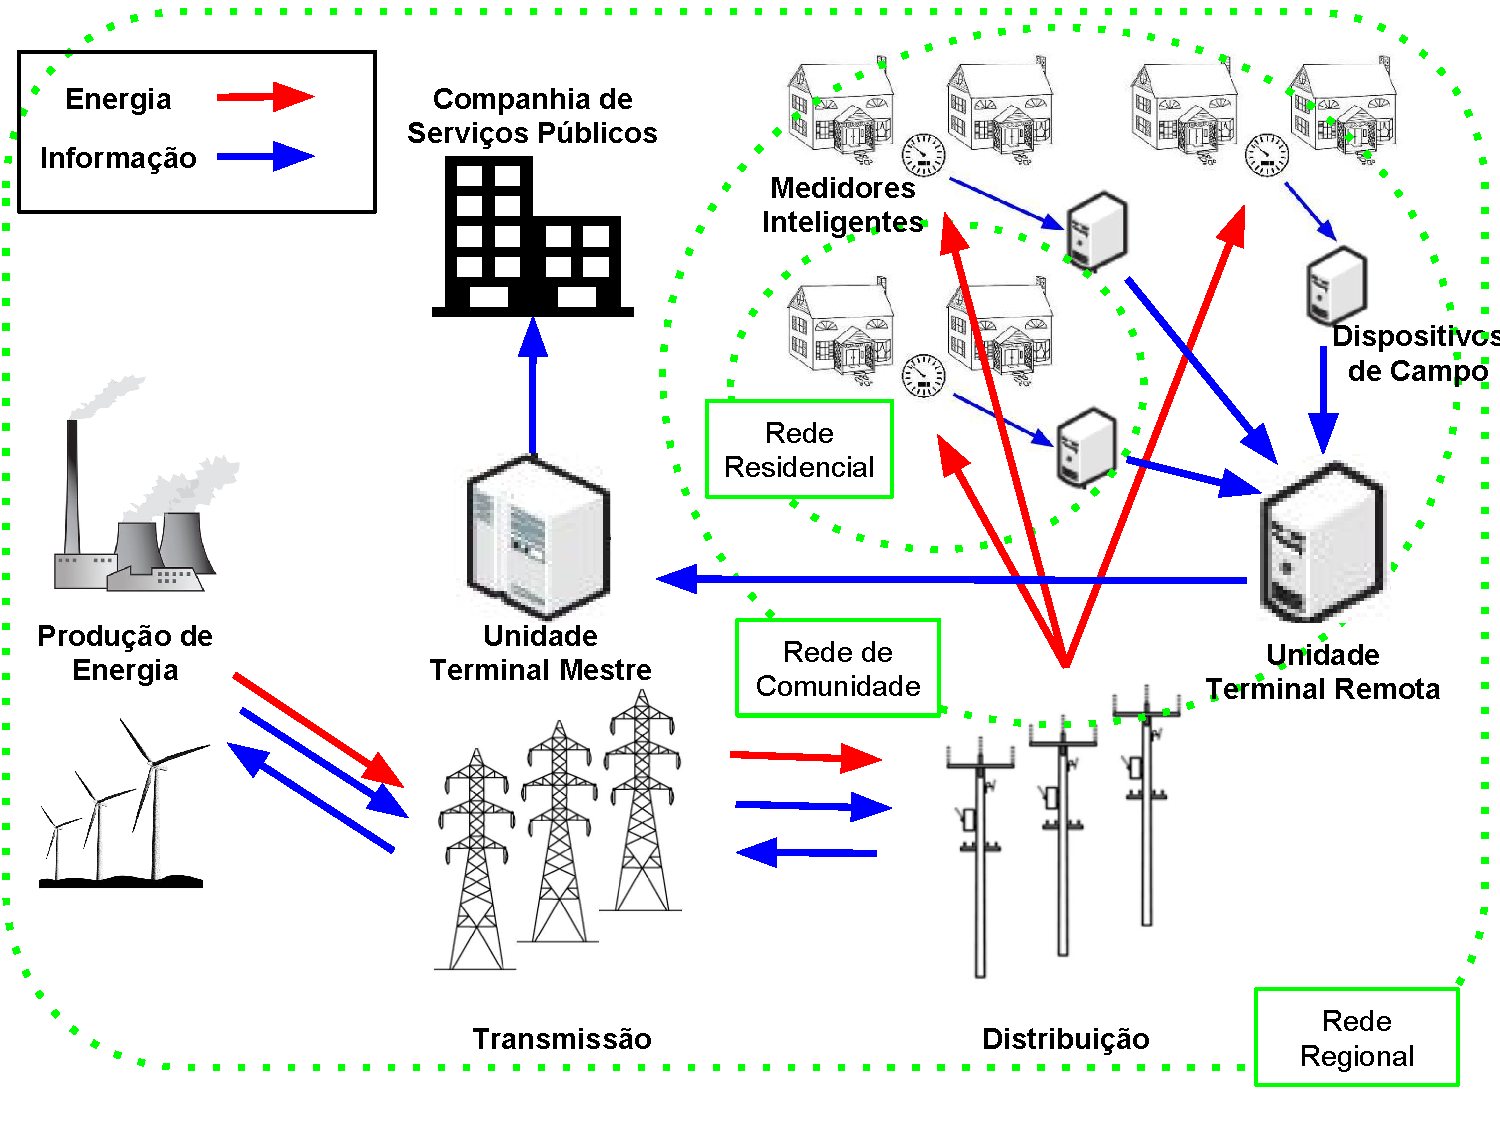
\includegraphics[width=30em]{smart_grid_arch}
   \end{center}
   \legend{Fonte: Autor}
   \label{fig:sgarchitecture}
\end{figure}

\subsubsection{Protocolos SCADA}

Os protocolos de comunicação utilizados em sistemas SCADA são projetados para garantir confiabilidade, operações em tempo real preciso e eficiência na comunicação entre componentes. Funções que prejudicam sua eficiência, incluindo funções de segurança, são desconsideradas na sua implementação, tornando-os menos seguros contra ameaças. Entre os diversos protocolos disponíveis para comunicação em sistemas SCADA, os mais amplamente utilizados são o Modbus e o DNP3 \cite{drias2015taxonomy}.

O Modbus é um protocolo do nível de aplicação, baseado no padrão requisição/resposta, desenvolvido para comunicação em tempo real entre controladores e dispositivos remotos. Apesar de inicialmente operar apenas sobre canais seriais, o protocolo foi estendido para funcionar em redes TCP/IP. Uma mensagem Modbus é composta por um cabeçalho de Protocolo de Aplicação Modbus, seguido por uma Unidade de Dados de Aplicação - \emph{Application Data Unit (ADU)} do Modbus. O cabeçalho é formado pelos campos:
\begin{itemize}
\item{Identificador de transação}: Permite o pareamento de requisições com suas respectivas respostas.
\item{Identificador de protocolo}: Identifica o protocolo de aplicação encapsulado pelo cabeçalho. O protocolo Modbus é identificado pelo código 0.
\item{Comprimento}: Tamanho, em bytes, da ADU.
\item{Identificador de unidade}
\end{itemize}
A UDA é formada por um código de função, que indica o tipo de transação presente na mensagem, e uma área de dados. A mensagem Modbus é encapsulada no pacote TCP, e enviada do cliente para o servidor pela porta 502 \cite{drias2015taxonomy}.

O DNP3 é um protocolo do nível de aplicação que implementa o modelo de comunicação mestre/escravo, desenvolvido para possibilitar uma comunicação confiável entre dispositivos SCADA geograficamente distribuídos. Surgiu como um protocolo serial, mas foi estendido para redes TCP/IP e UDP/IP. Para garantir a confiabilidade do protocolo, CRCs são utilizados em todas as trocas de mensagens entre o terminal mestre SCADA e os dispositivos remotos, que são os escravos. O protocolo DNP3 suporta fluxos de comunicação bidirecionais, permitindo que dispositivos remotos iniciem comunicação com o mestre. Apesar do protocolo DNP3 atualmente suportar Autenticação por Chave Compartilhada e Autenticação Baseada em Certificado, a falta de tecnologias padronizadas de gerenciamento de chaves em sistemas SCADA faz com que sejam pouco utilizados \cite{drias2015taxonomy}.

Outros protocolos, utilizados em menor escala em sistemas SCADA, incluem o IEC 60870-5-101, publicado no padrão IEC TC57 para controle de telecomunicações \cite{liguo2010iec}, o IEC 60870-5-104, uma evolução do IEC 60870-5-101 que inclui a comunicação com redes TCP/IP \cite{yang2014stateful} e o PROFIBUS, definido pelo padrão europeu EN50170 para automação industrial, monitoramento e comunicação de dados e controle de dispositivos de campo \cite{chen2011realtime}.

\subsection{Ameaças}
\label{subsecthreats}
A introdução de uma estrutura de comunicação autônoma e amplamente distribuída que ampara todo o funcionamento da rede elétrica expõe todo o sistema à possibilidade de ataques cibernéticos. A infraestrutura de comunicação, por ser desenvolvida sobre ICT, é inerentemente vulnerável a diversos tipos de ataque, que podem ser utilizados para manipular dados ou obstruir o funcionamento do sistema \cite{pin2012smart}. Medidores inteligentes também são potencialmente inseguros, estando vulneráveis a ataques de negação de serviço, roubo de informações de usuários e manipulação de dados \cite{ashford2011smartmeter}.

A evolução dos ataques cibernéticos e o risco que representam para infraestruturas críticas podem ser observados em fenômenos como o Stuxnet, um \textit{malware} desenvolvido para atacar controladores de sistemas industriais. O Stuxnet insere código ilegítimo na execução do controlador, que passa a ser executado em detrimento do código original, sem ser detectado, podendo levar à interrupção do serviço e danificar componentes do sistema atingido \cite{langner2011stuxnet}.

Uma taxonomia dos tipos de ataques cibernéticos em estruturas de comunicação de smart grids é apresentada em \cite{li2012securing}. Os autores descrevem quatro tipos de ataques: ataques a dispositivos, ataques de dados, ataques de privacidade e ataques de disponibilidade de rede.

\begin{itemize}
\item{Ataques a dispositivos}: Ataques a dispositivos têm como finalidade obter controle sobre um elemento do smart grid e utilizá-lo para um objetivo malicioso. De modo geral, servem a dois propósitos: fornecer os meios para um ataque de dados ou de disponibilidade ou, caso o dispositivo afetado possua funções de controle críticas, causar danos físicos ao sistema.
\item{Ataques de dados}: Ataques de dados configuram a tentativa de manipular os dados presentes na rede. Os dados manipulados podem ser informações de usuários ou sinais dos dispositivos de controle do smart grid. Seus usos variam de alterar dados de um usuário, para reduzir o valor da energia consumida, a eliminar sinais enviados por dispositivos de controle, para impedir o monitoramento e diagnóstico dos elementos da rede, o que pode levar à interrupção do funcionamento do sistema.
\item{Ataques de privacidade}: Ataques de privacidade têm o objetivo de obter informações privativas dos usuários. No caso dos smart grids, essas informações são os dados sobre o consumo de energia elétrica dos usuários, transmitidos pela rede de comunicação. Essas informações podem ser utilizadas para mapear dados privativos sobre a rotina dos usuários, que podem ser utilizados para fins maliciosos.
\item{Ataques de disponibilidade}: Ataques de disponibilidade de rede, ou ataques de negação de serviço, causam lentidão no tráfego de dados do smart grid através da sobrecarga da rede de comunicação e recursos computacionais. A velocidade da troca de dados é crítica para o funcionamento de um smart grid, e lentidão ou indisponibilidade do tráfego da rede podem causar prejuízos sérios aos seus usuários.
\end{itemize}

\section{Mecanismos de Detecção de Intrusão}
\label{secmec}
Garantir confiabilidade e segurança é um grande desafio no desenvolvimento dos smart grids. O desacoplamento das funcionalidades de controle e comunicação dos dispositivos elétricos e a modularização dos subsistemas leva a uma inevitável perda de confiabilidade. Componentes passam a ser originários de diferentes fabricantes, introduzindo margem à incompatibilidades e falhas de comunicação. A agregação de fontes de energia distribuída, incluindo usinas de geração instáveis, levam a fluxos de energia reversos e variações de voltagem. Ataques maliciosos podem ser direcionados tanto à rede elétrica física quanto à rede de comunicação \cite{li2012securing}. Apesar da existência de uma vasta gama de tecnologias de segurança voltadas à ICT, essas medidas de segurança não são capazes de resguardar o sistema contra ataques desenvolvidos para atingir sistemas SCADA, medidores inteligentes e outros componentes do smart grid \cite{carcano2011multidim}.

Sistemas de Detecção de Intrusão - \emph{Intrusion Detection Systems (IDSs)} são aptos a detectar ataques lançados através de dispositivos internos do sistema que tenham sido comprometidos, reconhecendo o comportamento padrão de um sistema e identificando ataques a partir da premissa de que as ações de um atacante diferem do funcionamento convencional do sistema \cite{li2012securing}. IDSs são caracterizados, de maneira geral, em doi tipos: Sistemas de Detecção de Intrusão baseados na Rede - \emph{Network based Intrusion Detection Systems (NIDSs)} e Sistemas de Detecção de Intrusão baseados no Hospedeiro - \emph{Host based Intrusion Detection Systems (HIDSs)}.

NIDSs são posicionados em pontos estratégicos ao longo da rede, afim de inspecionar o tráfego de dados entre todos os seus componentes. Os dados de tráfego podem ser, então, comparados a perfis de ataques maliciosos, para definir se os dados registrados se identificam com algum perfil de ataque conhecido, ou comparados a dados de tráfego normal da rede, com o objetivo de identificar tráfego anômalo, que pode indicar a ocorrência de um ataque. HIDSs são instalados em dispositivos individuais dentro da rede, e analisam o fluxo do tráfego que chega àquele componente. Assim como no NIDS, os dados de tráfego coletados são utilizados para identificar tráfego anômalo ou possíveis ataques.

Ao identificar tráfego anômalo ou possíveis ataques maliciosos, a principal tarefa do IDS consiste em registrar informações sobre os dados detectados e enviar um alerta para a central de controle do sistema. Sistemas de Detecção e Prevenção de Intrusões (SDPIs) são implementações de IDSs que utilizam técnicas para tentar suprimir ou bloquear ataques ao identificar tráfego suspeito. Entretanto, aplicar técnicas de prevenção de intrusão, que comumente consistem em desativar ou isolar o dispositivo sob ataque, pode ser complexo e arriscado em sistemas de infraestrutura crítica, que demandam alta disponibilidade.

A seguir, são discutidas as técnicas de detecção utilizadas em IDSs. A Seção \ref{detectiontec} descreve a taxonomia dos métodos de deteção de instrusão. Na Seção \ref{mldetection}, é discutido o uso de algoritmos de aprendizado de máquina para a classificação de tráfego, e é introduzido o algoritmo SVM, utilizado na implementação do IDS proposto neste trabalho. Por fim, a Seção \ref{scadaids} aborda técnicas utilizadas para a detecção de intrusão em sistemas SCADA.

\subsection{Detecção de Intrusão}
\label{detectiontec}
Em \cite{axelsson2000intrusion}, os mecanismos de detecção utilizados em IDSs são classificados em Detecção Baseada em Assinaturas - \emph{Signature Based Detection (SBD)} e Detecção Baseada em Anomalias - \emph{Anomaly Based Detection (ABD)}. Técnicas de SBD consistem em armazenar perfis de ataques maliciosos conhecidos, sem conhecimento do comportamento normal do sistema. Ao realizar a análise do tráfego, as informações são comparadas com os perfis de ataques existentes, a fim de identificar ameaças conhecidas. Métodos utilizados em SBD incluem:
\begin{itemize}
\item{Detecção baseada em regras - \emph{Rule-based detection}}: Utiliza regras simples para descrever o comportamento do sistema sob um ataque. Quando os dados detectados se enquadram nas regras descritas, a intrusão é detectada.
\item{Modelagem de estados - \emph{State-moddeling}}: Modela o comportamento do sistema através de uma máquina de estados, onde determinadas sequências de transições entre os estados identificam a intrusão.
\item{Reconhecimento de texto - \emph{String matching}}: Reconhece sequências de caracteres pré-definidas como  comportamento intrusivo nos dados enviados e recebidos pelo sistema, ou em dados resultantes de processamentos do sistema.
\item{Sistema especialista - \emph{Expert system}}: É uma forma mais avançada da detecção baseada em regras. Utiliza uma série de regras e critérios, que descrevem uma situação de intrusão, para ponderar sobre o estado atual do sistema. São mais flexíveis que os métodos mais simples, porém com maior complexidade e menor performance.
\end{itemize}

Mecanismos de ABD se baseiam em reconhecer o comportamento normal esperado do sistema. Ao monitorar o tráfego da rede, os dados analisados são classificados em tráfego normal, se são condizentes com o comportamento esperado do sistema, ou anormal, se diferem do comportamento esperado. Em geral, os métodos utilizados para ABD são:
\begin{itemize}
\item{Detecção programada - \emph{Programmed detection}}: Informações são inseridas no detector para que ele reconheça o comportamento normal do sistema, e modelar, através de regras ou de máquinas de estados, os critérios para que o comportamento seja considerado anormal.
\item{Sistemas de auto-aprendizado - \emph{Self-learning systems}}: O detector aprende através de exemplos a reconhecer o comportamento normal do sistema, observando o sistema em funcionamento por um período de tempo e construindo um modelo a partir dos dados coletados. Esta técnica utiliza modelos de detecção mais complexos, gerados por algoritmos de aprendizado de máquina. 
\end{itemize}

Mecanismos de SBD são capazes de identificar de forma mais eficiente ameaças conhecidas ao sistema do que mecanismos de ABD, que visam apenas identificar tráfego de dados anômalo, de forma geral. Entretanto, a implementação de SBD necessita de dados específicos e precisos sobre cada ataque que terá um perfil incluído para identificação. Esses dados podem ser difíceis de obter para alguns sistemas, pois suas informações podem não estar disponíveis. Além disso, não é possível listar exaustivamente todos os ataques que podem ser lançados à um sistema, já que ataques existentes podem ser modificados e novos ataques podem surgir a qualquer momento. Dessa forma, mecanismos de SBD geralmente são utilizados como complemento para mecanismos de ABD, que podem ser implementados com conhecimento apenas sobre o tráfego normal do sistema.

\subsection{Classificação de Tráfego com Algoritmos de Aprendizado de Máquina}
\label{mldetection}

A implementação de um IDS baseado em Detecção de Anomalias requer a realização da classificação, durante a execução, do tráfego de dados do sistema. Algoritmos de Aprendizado de Máquina - \emph{Machine Learning (ML)} têm sido utilizados para a classificação de tráfego de dados por por possuírem diversas características vantajosas para a tarefa. Enquanto técnicas de classificação de tráfego tradicionais dependem da inspeção do conteúdo de pacotes, mecanismos baseados em ML classificam os dados através de atributos que podem ser observados externamente, como tamanho dos pacotes e tempo entre a chegada de pacotes, criando padrões estatísticos. Há benefícios consideráveis nessa abordagem: o campo de dados do pacote deixa de ser obrigatoriamente visível  (os dados podem estar criptografados, por exemplo), e o classificador não precisa conhecer a sintaxe dos dados nos pacotes de cada aplicação \cite{nguyen2008survey}. Os algoritmos de ML podem ser classificados em duas categorias:

\begin{itemize}
\item{Aprendizado supervisionado}: No aprendizado supervisionado, o algoritmo é treinado utilizando um conjunto de instâncias já classificadas, rotuladas com classes pré-definidas. O modelo gerado no treinamento é utilizado para classificar um conjunto de instâncias desconhecidas. Um algoritmo de aprendizado supervisionado é composto por duas fases principais. Na fase de treinamento, o algoritmo analisa o conjunto de instâncias de trinamento, já classificadas, e identifica relações entre os atributos e as classes, a fim de gerar um modelo de regras para a classificação. Na fase de teste, o modelo gerado durante a fase de treinamento é utilizado para identificar a classe de novas instâncias, ainda não classificadas. Existe uma vasta gama de algoritmos de aprendizado supervisionado, um exemplo sendo o algoritmo de classificação \emph{Naive Bayes}.
\item{Aprendizado não supervisionado}: Algoritmos de aprendizado não supervisionado não possuem uma fase de treinamento com classes já definidas. Em vez disso, implementam heurísticas para descobrir padrões entre os dados das instâncias e agrupá-las em \emph{clusters} com características similares. Os grupos podem ser exclusivos, quando uma intância não pode pertencer a mais de um grupo, ou sobrepostos, quando as instâncias podem pertencer a diversos grupos. Os principais métodos de aprendizado não supervisionado são os algoritmos \emph{k-means}, clusterização incremental e clusterização baseada em probabilidade.
\end{itemize}

Segundo \cite{nguyen2008survey}, a tarefa de classificação de tráfego utilizando ML requer, primeiramente, que atributos sejam definidos. Atributos são características dos fluxos de pacotes entre os dispositivos da rede, como tamanho máximo e mínimo de pacote e tempo médio entre chegada de pacotes, que serão utilizados para selecionar instâncias de dados de tráfego. É necessário, então, treinar o algoritmo classificador, associando conjuntos de atributos com classes de tráfego definidas. Através da etapa de treinamento, o algoritmo gera o conjunto de regras que será utilizado para determinar a qual classe pertence uma determinada entrada. Finalmente, utilizando o modelo gerado no treinamento, o classificador pode receber dados de tráfego desconhecidos e identificar a que classe pertencem. 

Máquina de Vetores de Suporte - \emph{Support Vectors Machine (SVM)} é um algoritmo de ML, definido em \cite{cortes1995support}, baseado em aprendizado supervisionado e amplamente utilizado para a tarefa de classificação de dados. O algoritmo utiliza um conjunto de dados previamente classificados, chamado conjunto de treinamento, para definir um modelo de classificação, que utiliza regras geradas durante o treinamento para prever a que classe pertencem instâncias de dados desconhecidas. O SVM considera cada instância de dados como um vetor de \emph{n} dimensões, e o modelo de classificação é construído de forma a separar as instâncias em suas respectivas classes com um único hiperplano de \emph{n-1} dimensões. A solução clássica do SVM encontra o hiperplano linear com a maior margem possível entre as classes. Entretanto, o SVM permite a utilização de funções de kernel não lineares, possibilitando gerar modelos com hiperplanos não lineares, que ampliam a distância máxima da margem entre as classes.

\subsection{IDSs em sistemas SCADA}
\label{scadaids}
Existe uma ampla variedade de IDSs voltados para redes de comunicação tradicionais. Todavia, IDSs desenvolvidos para ICT falham em suprir os requisitos de segurança de sistemas SCADA, e mecanismos voltados para satisfazer as necessidades desses sistemas ainda não estão suficientemente amadurecidos. Portanto, novos mecanismos para detecção de ameaças devem ser desenvolvidos especificamente para a rede de sistemas SCADA.

Em \cite{coutinho2009anomaly}, os autores apresentam uma técnica de detecção de anomalias para centros de controle de infraestruturas críticas, utilizando o Algoritmo de Classificação de Conjuntos Irregulares - \emph{Rough Sets Classification Algorithm}. O algoritmo foi capaz de identificar dados corrompidos introduzidos em um sistema de energia elétrica de seis barramentos. Uma abordagem à detecção de intrusão em sistemas SCADA baseada em Análise de Estado Crítico e Proximidade de Estados é analisada em \cite{carcano2011multidim}. Um IDS multiagente é introduzido em \cite{tsang2005multi}, baseado no Modelo de Clusterização da Colônia de Formigas - \emph{Ant Colony Clustering Model}, para detecção descentralizada de anomalias em redes distribuídas. Os resultados obtidos apresentam alta acurácia na detecção e baixa taxa de falsos positivos. Em \cite{yang2013iecdetection}, os autores propõe e avaliam um IDS baseado em SBD para sistemas SCADA que utilizam o protocolo IEC 60870-5-104, utilizando um conjunto de regras para a identificação de ameaças conhecidas, e obtém resultados positivos nos testes com identificação de ameaças. Um framework para a detecção de intrusões e apresentado em \cite{2014multiattribute}, que utiliza um sistema hierárquico para incluir IDSs distribuídos ao longo da estrutura do sistema SCADA. O framework utiliza regras e perfis para analisar o comportamento da rede, e os testes realizados obtiveram sucesso na detecção de ataques cibernéticos inseridos no sistema SCADA. Em \cite{2014temporalintrusion}, um IDS específico para sistemas SCADA é proposto baseado na identificação de relações de tempo entre os pacotes da rede. O IDS foi testado utilizando dados reais do sistema SCADA uma usina de energia, e os resultados obtiveram uma taxa alta de identificação de ameaças com poucos falsos positivos. Já em \cite{aliprobabilistic}, os autores propõe um IDS para AMIs, coletando dados do AMI e modelando seu comportamento para comparação com especificações de configuração dos dispositivos. Os resultados são validados utilizando dados reais obtidos de medidores de uma AMI, obtendo uma alta taxa de detecção. Por fim, o framework AMIDS é apresentado em \cite{mclaughlinamids} para a detecção de intrusão em AMIs, combinando registros de medição com dados de consumo para modelar o comportamento do AMI. Nos testes realizados, o framework identificou com sucesso tentativas de roubo de energia.

\section{Ferramentas de Simulação}
\label{sectools}

A fim de realizar a implementação e a avaliação do IDS proposto neste trabalho, é necessário utilizar uma ferramenta que permita a simulação da estrutura de comunicação de um smart grid. São apresentadas, a seguir, algumas ferramentas que possibilitam a simulação de tráfego de dados entre componentes SCADA. Algumas ferramentas suportam apenas simulações do fluxo de dados em componentes específicos, como o PLC, enquanto outras permitem a simulação de estruturas mais completas, com tráfego de dados entre diversos componentes.


\subsection{VirtuaPlant}
VirtuaPlant \cite{virtuaplantwebsite} é um simulador de Sistemas de Controle Industriais (SCI). Possui uma interface gráfica chamada World View que simula o efeito das ações do sistema de controle sobre um recurso virtual utilizando protocolo Modbus. O recurso é representado por uma fábrica que enche garrafas.
	
Um PLC é implementado sobre a biblioteca pymodbus, que roda em uma thread separada no componente World View e compartilha seu contexto, que contém registradores, entradas e valores, com as funções do World View para simular recursos sendo conectados ao controlador. A Interface Homem-Máquina (IHM) utiliza GTK3 e executa o cliente pymodbus em uma thread separada, que conecta com o servidor através de TCP/IP, obtendo leituras constantes dos valores do servidor, isto é, do PLC.

A ferramenta VirtuaPlant fornece uma variedade de scripts de ataque ao PLC. Entretanto, não permite a definição de novos dispositivos, não sendo possível a definição de novas topologias. Também não possibilita a modelagem de elementos da infraestrutura de comunicação, já que a simulação engloba apenas a leitura e escrita dos valores do controlador PLC.

\subsection{mosaik}
O mosaik \cite{mosaikwebsite} permite usar diversos simuladores existentes em um contexto comum para realizar uma simulação coordenada de um cenário, que representa um conjunto de componentes de smart grid. Oferece uma API para os simuladores se comunicarem com ele e possui handlers para cada tipo de processo dos simuladores.
	
A ferramenta permite a modelagem de diferentes cenários envolvendo esses simuladores, possibilitando a criação de novos objetos e definição de novas topologias. A biblioteca SimPy é utilizada para a simulação coordenada de cenários, e a execução da simulação é feita executando passos em cada simulador ao longo do tempo. Cada simulador executa o seu próprio processo e laço de eventos, enquanto o Mosaik sincroniza esses processos e gerencia a troca de dados entre eles. Através da combinação com outros simuladores, é possível simular uma estrutura ICT.

O protocolo de comunicação entre o mosaik e os simuladores é definido por uma API. Existem duas versões da API: alto nível e baixo nível. A API baixo nível utiliza sockets TCP para estabelecer a comunicação entre o mosaik e os simuladores através da troca de mensagens JSON. A API alto nível, atualmente disponível nas linguagens Python e Java, fornece o encapsulamento dessa comunicação em uma classe abstrata, onde as mensagens trocadas entre os simuladores e o mosaik são implementadas como métodos.

A criação de cenários de simulação é feita por uma API que permite iniciar simuladores e instanciar modelos a partir deles, criando um conjunto de entidades. É possível conectar as entidades entre si para estabelecer a troca de dados entre elas.

O gerenciador de simuladores é responsável por iniciar e gerenciar os processos dos simuladores e a comunicação entre eles. Permite iniciar novos processos de simuladores, conectar a processos que já estão em execução e, no caso de simuladores desenvolvidos em Python, também permite importar módulos de simuladores e executá-los durante a execução do processo.

Em \cite{wermann2015astoria}, os autores apresentam o framework ASTORIA, desenvolvido a partir da integração do mosaik com um simulador de redes, que permite a especificação e execução de simulações customizadas de ambientes smart grids. Além disso, permite definir ataques, como Negação de Serviço - \emph{Denial of Servie (DoS)}, ao ambiente simulado e avaliar seu impacto na estrutura do smart grid.

\subsection{SCADASim}
A ferramenta SCADAsim \cite{scadasimart} é um framework para construção de simulações SCADA. Possui um conjunto de módulos que representam os componentes SCADA, como RTUs, PLCs e MTUs, e implementa os protocolos Modbus TCP e DNP3. Permite a integração de componentes externos e componentes internos simultaneamente através do conceito de Gates, que são objetos que conectam um ambiente externo com o ambiente da simulação.

É baseado em 3 componentes principais: SSScheduler, SSGate e SSProxy.  SSScheduler é um escalonador em tempo real que permite controlar e sincronizar mensagens recebidas. Gerencia uma lista de instâncias do componente SSGate, que são responsáveis por enviar e receber mensagens de um ambiente externo, garantindo a sincronização das mensagens entre dois ambientes. SSGate fornece conexão com o ambiente externo através de um protocolo, que é utilizado para se comunicar com os componentes SCADA externos. Atualmente os protocolos disponíveis são: ModbusGate, DNP3Gate e HTTPGate. SSProxy representa um dispositivo real ou aplicação externa que interage com os objetos simulados e com um SSGate, que direciona suas mensagens para componentes externos.

Os protocolos são gerenciados de dois modos. Os protocolos utilizados dentro do ambiente do simulador para comunicação entre componentes da simulação são chamados de protocolos simulados. Os protocolos utilizados para comunicação entre dispositivos e aplicações externas e os SSGates são chamados de protocolos originais. No ambiente interno da simulação, toda a comunicação entre os componentes utiliza versões simuladas dos protocolos SCADA. O framework possui uma biblioteca de protocolos SCADA originais e simulados, contendo: Modbus TCP, DNP3 TCP e HTTP.

O simulador SCADASim permite, através dos módulos integrados de componentes SCADA, criar componentes e definir topologias, além de possibilitar a integração com componentes reais através da API. Possui, também, uma biblioteca com alguns tipos de ataques comuns à estruturas SCADA, como worm e DDoS. Não suporta, todavia, a modelagem de elementos de geração de energia, presentes em um smart grid.

\subsection{Modbus PLC Simulator}
O Modbus PLC Simulator \cite{plcsimwebsite} é um simulador de PLC baseado na ferramenta Modbus Slaves. O Modbus Slaves é uma ferramenta que permite simular até 32 dispositivos simultaneamente. Os dados contidos nos dispositivos escravos (slaves) são acessíveis à aplicação mestre. Permite monitoramento de tráfego serial. Cada instância de escravo pode ser configurada para representar dados de um mesmo nodo ou de nodos diferentes.

A ferramenta suporta os protocolos Modbus TCP/IP, Modbus RTU (serial) e AB-DF1. Funciona criando uma thread de comunicação com interface para a API de comunicação e controla um bloco de RAM que funciona como a memória do PLC.

O Modbus PLC Simulator possibilita a simulação da troca de dados entre um dispositivo PLC, representado pela aplicação mestre, e outros dispositivos, não fornecendo suporte, entretanto, para os demais aspectos da comunicação ICT, como modelagem de topologias e de dispositivos da infraestrutura de rede.


\subsection{Comparação entre ferramentas de simulação}

O IDS visa realizar a detecção de anomalias em uma rede SCADA através da classificação dos dados de tráfego em tempo real. Para que esta solução seja possível, o único requisito estritamente necessário à escolha da ferramenta a ser utilizada é que ela deve ser capaz de simular o tráfego de dados entre componentes de uma estrutura SCADA. Caso contrário, não será possível realizar a classificação do tráfego entre componentes. Dito isso, outras características são interessantes para realizar uma simulação mais completa, que gere cenários mais próximos a um smart grid real, como a modelagem de componentes, a definição de topologias e a possibilidade de definir ataques para a simulação. A Tabela \ref{tbl:comparacaosim} apresenta uma comparação entre as ferramentas de simulação previamente abordadas utilizando os seguintes critérios:

\begin{itemize}
\item{Simulação da infraestrutura ICT}: A ferramenta permite a simulação de uma estrutura ICT. É um requisito obrigatório da ferramenta a ser escolhida, pois é necessário simular o tráfego de dados entre componentes SCADA.
\item{Simulação de produção e consumo de energia}: A simulação de valores de produção e consumo de energia permite que o ambiente simulado seja mais próximo ao ambiente real de um smart grid.
\item{Elementos modeláveis}: Quais elementos da simulação podem ser modelados. Quanto maior a flexibilidade para modelar elementos, mais próxima à estrutura de um smart grid podemos tornar a simulação.
\item{Protocolos de rede} A utilização de um dos protocolos comumente utilizados em redes de comunicação SCADA torna possível classificar os dados de tráfego de forma similar a um smart grid real.
\item{Modelagem de troca de pacotes de rede e informações de energia}: Como é realizada a modelagem do tráfego de dados e do fluxo de energia elétrica na simulação. Idealmente, a modelagem deve ter um grau de abstração que torne o uso da ferramenta simples.
\item{Definição de novas topologias} A possibilidade de definir novas topologias possibilida a simulação de cenários com configuração semelhante à de um smart grid.
\item{Criação e simulação de ataques} Definir e executar ataques sobre a estrutura simulada é uma maneira eficiente de avaliar o IDS a ser implementado.
\end{itemize}

\begin{table}[h]
    \caption{Comparação entre ferramentas de simulação}
    % OBS: não use \begin{center}, pois este aumenta o espaçamento entre a caption/legend e a tabela
    % Para figuras, a aparência é melhor com o espaçamento extra
    \centering
    \scriptsize
    % \setstretch{0.8}
        \begin{tabular}{m{2.4cm}|m{2.4cm}|m{2.4cm}|m{2.4cm}|m{2.4cm}}
          \hline
           & \textit{VirtuaPlant} & \textit{mosaik} & \textit{SCADASim} & \textit{Modbus PLC Simulator} \\
          \hline
          \hline
          Simulação da infraestrutura ICT & N/D & API permite integração com simuladores de rede & Componente SSGate simula estrutura de comunicação & N/D \\
          \hline
          Simulação de produção e consumo de energia & N/D & Modelado pelo simulador PYPOWER & N/D & N/D \\
          \hline
          Elementos modeláveis & Leitura e escrita de valores do PLC & Infraestrutura SCADA, topologia da rede, consumo e geração de energia & Infraestrutura SCADA & Apenas tráfego de dados entre componentes e PLC \\
          \hline 
          Protocolos de rede & Modbus & API para integração com simuladores de rede & Modbus e DNP3 & Modbus \\
          \hline
          Modelagem de troca de pacotes de rede e informações de energia & N/D & 	Através dos simuladores de rede integrados & Modelagem realizada pelo componente SSGate & N/D \\
          \hline
          Definição de novas topologias & N/D & Permite definição de componentes e topologias & Permite definição de componentes e topologias & N/D \\
          \hline
          Criação e simulação de ataques & Inclui ataques que atingem os dados do PLC & Framework ASTORIA inclui definição e simulação de ataques à estrutura SCADA & Inclui biblioteca de ataques a componentes da estrutura SCADA & Possível desenvolver ataques para o componente PLC \\
          \hline
        \end{tabular}
    \legend{Fonte: Autor}
    \label{tbl:comparacaosim}
\end{table}

A partir da comparação entre as ferramentas, é possível analisar qual é mais adequada para o propósito deste trabalho. Apesar de permitirem a leitura e escrita de dados em componentes SCADA, os simuladores VirtuaPlant e Modbus PLC Simulator não possibilitam a simulação da infraestrutura ICT presente em um smart grid. Ambos os simuladores mosaik e SCADASim permitem a simulação da infraestrutura ICT do sistema SCADA, a definição de novas topologias e a modelagem de seus componentes de forma suficientemente simples. O mosaik, no entanto, permite a simulação da rede de energia elétrica presente em um smart grid, enquanto o SCADASim simula apenas a rede de comunicação.
Apesar de a simulação de um ambiente smart grid através do mosaik requisitar a integração com um simulador de redes, o framework ASTORIA implementa essa integração e permite a simulação tanto da rede elétrica quanto da rede de comunicação presentes em um smart grid, além de fornecer ataques que podem ser executados sobre a simulação. Deste modo, o framework ASTORIA foi escolhido como ferramenta para simulação do ambiente smart grid neste trabalho.

\chapter{Modelagem e Desenvolvimento}
O problema proposto por este trabalho consiste em implementar um mecanismo de detecção de intrusão e avaliá-lo utilizando uma ferramenta que simule a infraestrutura de um smart grid. Para isso, é necessário desenvolver um IDS e integrá-lo à ferramenta de simulação, de modo que o IDS possa receber, em tempo real, dados do ambiente smart grid e operar sobre eles.
 
Neste capítulo, serão apresentadas a modelagem e as ferramentas utilizadas para o desenvolvimento de uma solução para o problema proposto. A Seção \ref{secastoria} contém mais informações sobre o framework ASTORIA, utilizado para configurar as simulações do ambiente smart grid. A Seção \ref{secsdi} descreve a modelagem do IDS proposto e as tecnologias utilizadas para desenvolvê-lo.
 
\section{Simulação da estrutura de smart grid com Framework ASTORIA}
\label{secastoria}

O Framework ASTORIA, descrito pelos autores em \cite{wermann2015astoria}, permite modelar simulações de ambientes smart grid, definir e executar ataques nesses ambientes e avaliar seus resultados e o comportamento do sistema.
O propósito da utilização do mosaik é agregar diversos simuladores em um contexto comum, para que sua execução sincronizada possa criar um ambiente de smart grid. Para isso, é necessário conectar as ferramentas que farão a simulação dos componentes dos smart grid.
 
A simulação da rede elétrica é realizada pelo PYPOWER, uma ferramenta nativamente integrada ao mosaik. Para realizar a simulação do componente de comunicação do smart grid, foi realizada a integração do mosaik com o simulador de redes ns-3.

A seguir, é apresentado o framework ASTORIA, seu funcionamento e as simulações produzidas por ele. A Seção \ref{subsecinteg} descreve a integração entre as ferramentas que compõe o framework, os simuladores mosaik, ns-3 e PYPOWER. Na Seção \ref{subsecestrut}, são mostradas a estrutura das simulações produzidas pelo framework.

\subsection{Integração entre as ferramentas}
\label{subsecinteg}
 
A simulação de um smart grid utilizando o ASTORIA acontece através da integração das funcionalidades de três ferramentas: PYPOWER, que realiza a simulação da rede de energia elétrica, ns-3, que simula a rede de comunicação da estrutura SCADA, e mosaik, que sincroniza a execução das demais ferramentas.
 
O PYPOWER \cite{pypower},  é uma ferramenta que implementa as funcionalidades do MATPOWER \cite{matpower} na linguagem Python e permite simular cenários de fluxo de energia elétrica, fornecendo os dados de produtores e consumidores de energia. O PYPOWER permite a simulação de uma estrutura de rede elétrica e gera dados de produção e consumo em tempo real. Esses dados são fornecidos, através do mosaik, para a rede de comunicação. O fluxo de energia simulado pelo PYPOWER para cada nodo da rede elétrica é gerado a partir de perfis de produção e consumo de energia, já presentes na ferramenta. Como o PYPOWER já é originalmente integrado ao mosaik, os dois já estão conectados e não há necessidade de implementar a troca de dados entre eles.

O ns-3 \cite{nsnam}, utilizado para compor o elemento de comunicação da simulação do smart grid, é um simulador de redes que funciona mantendo uma lista de eventos que devem ser executados, sequencialmente, em determinados tempos da simulação.  Desenvolvido para fins de estudo e pesquisa, está disponível publicamente para uso, e sua estrutura suporta simulações tanto de redes baseadas em IP quanto de redes não baseadas em IP. Também permite a interação entre simulações e dispositivos reais, possibilitando o envio de pacotes gerados pelo simulador para dispositivos de uma rede real.
 
A integração do mosaik com o simulador ns-3, descrita em \cite{wermann2015astoria}, foi feita através da mosaik Sim API, que possibilita a sincronização com outros simuladores. A comunicação entre as ferramentas é realizada através de sockets TCP e mensagens  no formato JSON. As mensagens seguem o padrão requisição-resposta e são compostas por um cabeçalho, que carrega o número de bytes do corpo, e pelo corpo da mensagem, que contém o tipo, o identificador e o conteúdo da mensagem. O ns-3 inicia a conexão com o mosaik através de um socket TCP e, por meio dessa conexão, é realizado o envio das mensagens, através das quais o mosaik sincroniza a execução dos dois simuladores, PYPOWER e ns-3, e fornece os dados da rede elétrica para a rede de comunicação.
 
A execução do mosaik é baseada em passos. Após a fase de configuração, em que é feita a inicialização dos simuladores e a criação das instâncias de simulação, é enviada para o ns-3 uma mensagem a cada passo de execução, contendo os dados referentes à produção e ao consumo de energia, gerados pelo PYPOWER. Ao receber a mensagem contendo esses dados, o ns-3 executa a etapa atual da simulação, responde a mensagem com o instante em que a próxima etapa de simulação deve ser executada e entra em espera até receber a próxima mensagem.

\subsection{Simulação do ambiente smart grid}
\label{subsecestrut}

A rede de energia elétrica é composta por nodos de geração, consumo e distribuição de energia. Os dados de consumo de cada nodo são gerados pelo PYPOWER, que gera o fluxo de cada componente a partir de perfis de produção e consumo de energia presentes no simulador. A estrutura SCADA formada pela rede de comunicação é composta por sensores, RTUs e MTUs. Cada nodo de produção, distribuição e consumo presente na rede elétrica possui um nodo correspondente na rede de comunicação SCADA. Cada nodo de produção ou consumo está pareado com um sensor SCADA, enquanto os nodos de distribuição de energia estão pareados com as RTUs. As MTUs não possuem nenhum componente respectivo na rede elétrica, por serem um componente exclusivo da estrutura SCADA.

A Figura \ref{figsimulation} mostra a estrutura dos componentes na simulação do ambiente smart grid com o framework ASTORIA. A comunicação entre os componentes SCADA acontece através do protocolo modbus. O mosaik fornece a cada sensor SCADA as informações sobre o consumo de energia do nodo da rede elétrica associado a ele. A cada passo de execução, as RTUs enviam requisições para todos os sensores conectados a elas, e os sensores respondem enviando os dados de consumo obtidos. A MTU envia requisições para todas as RTUs, que enviam respostas contendo as informações recolhidas de toda a sua região. A topologia da simulação é definida por um arquivo de configuração em que são instanciados os componentes MTU, RTUs e sensores, e as conexões entre os componentes. Todas as RTUs são conectadas à MTU, e cada RTU possui um conjunto de sensores conectados a ela.

\begin{figure}[h]
   \caption{Estrutura da simulação com o framework ASTORIA}
   \begin{center}
       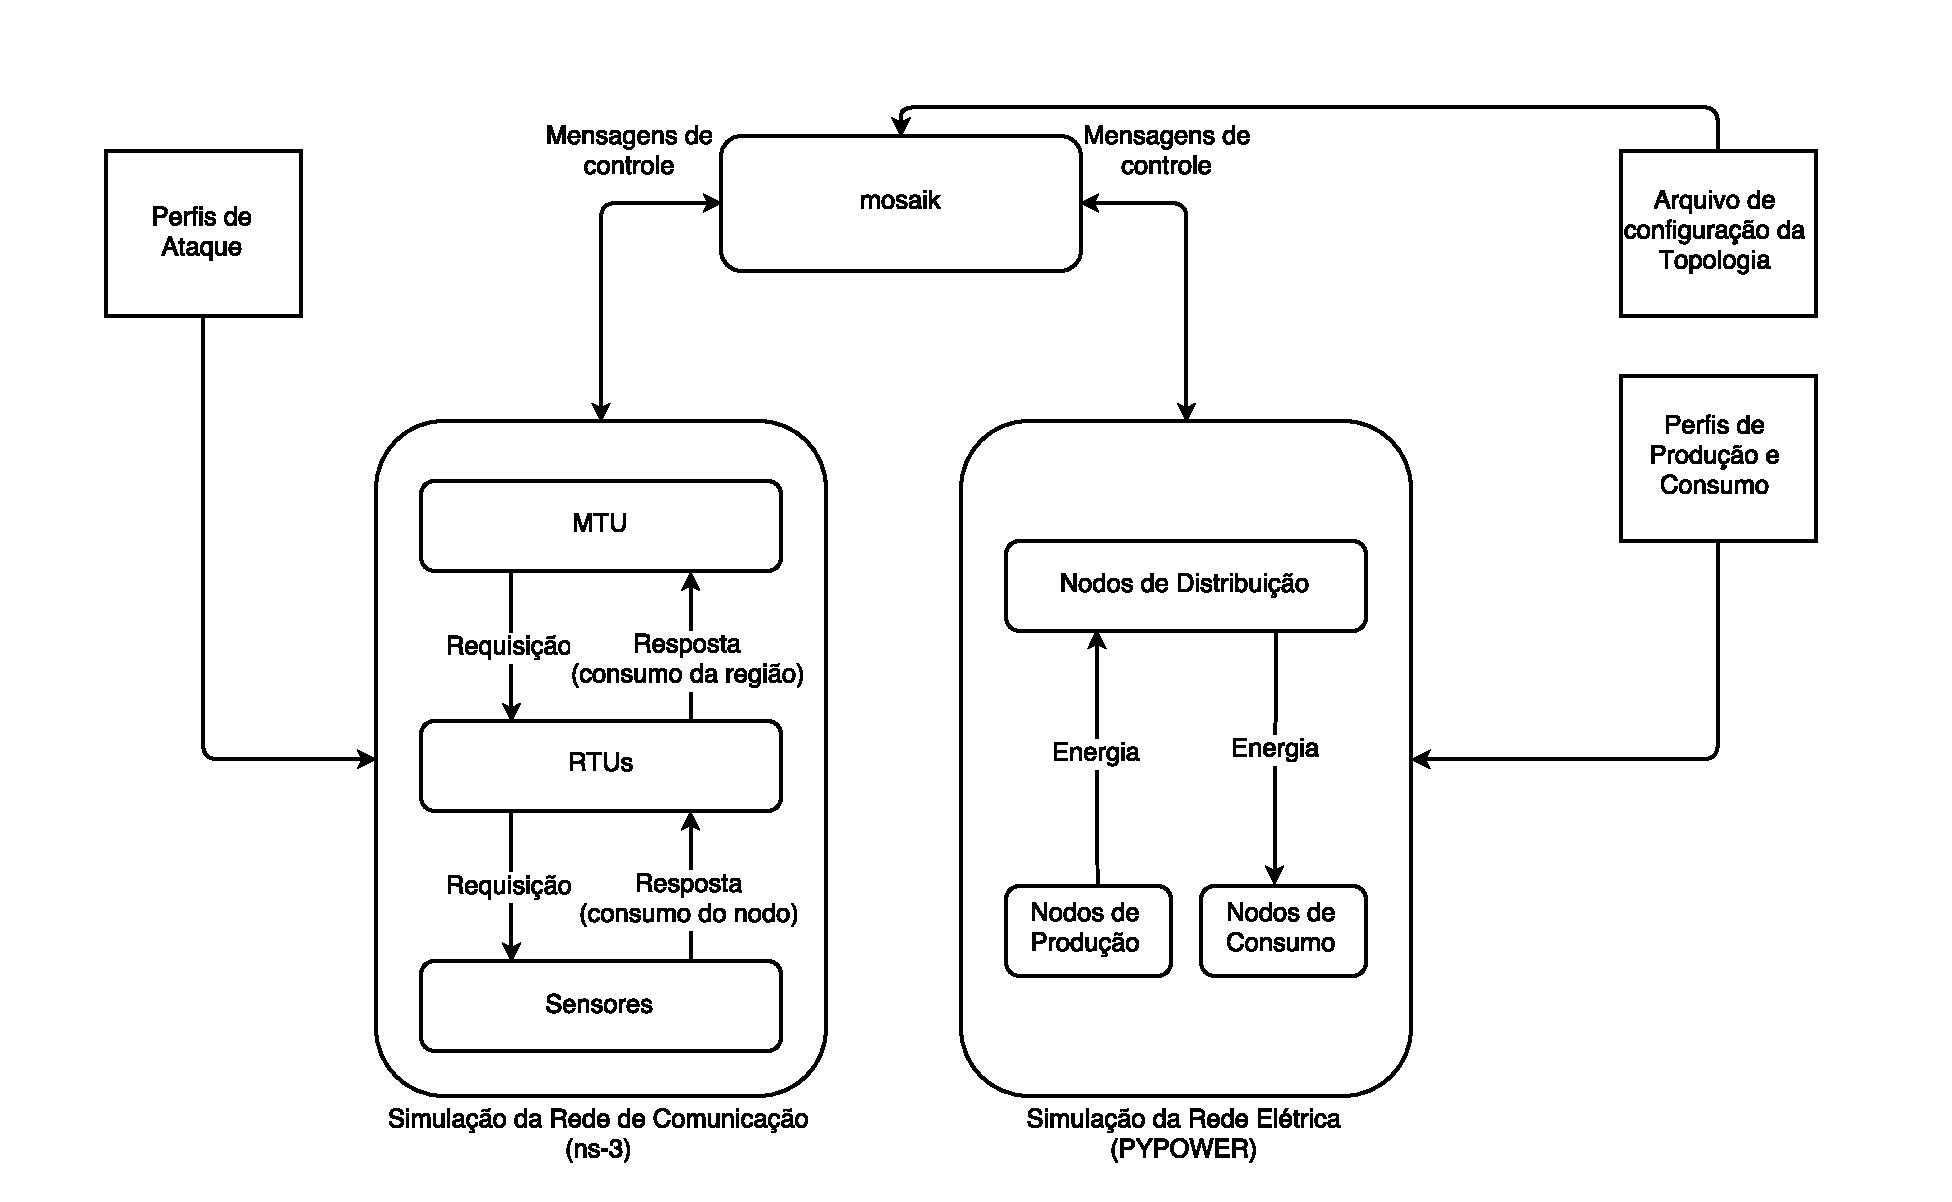
\includegraphics[width=30em]{astoria_simulation}
   \end{center}
   \legend{Fonte: Autor}
   \label{figsimulation}
\end{figure}

O framework ASTORIA também oferece uma biblioteca de ataques, que podem ser executados sobre a simulação do smart grid. Os ataques podem ser instanciados através de perfis, que permitem a configuração de diferentes tipos de ataques. Os perfis de ataques são compostos pelos parâmetros:
\begin{itemize}
\item{Tipo de Ataque}: Tipo do ataque definido no perfil, como Negação de Serviço - \emph{Denial of Service (DoS)}, que será executado na simulação.
\item{Nodo de Origem}: Nodo da simulação do qual se origina o ataque.
\item{Nodo Alvo}: Nodo da simulação que será atingido pelo ataque.
\item{Passo de Execução}: Define a frequência e a intensidade do ataque. Em um ataque DoS, por exemplo, o passo de execução pode ser definido como 4 milissegundos, indicando que o nodo atacado receberá 250 pacotes por segundo.
\item{Tempo de Início}: Horário de início do ataque na simulação.
\item{Parâmetros Específicos}: Uma lista de parâmetros opcionais, específicos para determinados tipos de ataques. O tamanho dos pacotes enviados pelo atacante, por exemplo, pode ser definido para um ataque que cause \emph{buffer overflow}.
\end{itemize}

O framework contém dois tipos de ataques definidos. O ataque DoS visa parar o funcionamento dos nodos atingidos através do envio de um grande volume de pacotes, e é implementado através de uma aplicação maliciosa que é instanciada nos nodos de origem, que recebe os parâmetros do perfil de ataque DoS. O ataque de Injeção de Software Malicioso é implementado por uma aplicação maliciosa que infecta uma RTU, também recebendo parâmetros do perfil de ataque correspondente. Quando dados da RTU infectada são requisitados pela MTU, a aplicação maliciosa responde informando dados de consumo incorretos para toda uma região. Entretanto, o framework e a biblioteca de ataques são extensíveis, e novos perfis de ataques podem ser definidos e implementados sobre a simulação do smart grid.
 
\section{Mecanismo de Detecção de Intrusão}
\label{secsdi}

A incorporação de um IDS no sistema SCADA de um smart grid permite a rápida identificação de situações de risco, como ataques cibernéticos, que podem comprometer o funcionamento correto do sistema. Ao detectar rapidamente anomalias no comportamento do sistema, é possível se beneficiar de medidas responsivas de segurança, minimizando os danos causados pelo ataque ao sistema. 

A seguir, são abordadas as técnicas utilizadas para o desenvolvimento do IDS implementado na ferramenta ASTORIA. Na Seção \ref{subsec:ocsvm}, é descrito o algoritmo Máquina de Vetores de Suporte de Uma Classe, utilizado neste trabalho, e a Seção \ref{subsec:sdimodel} apresenta a modelagem do IDS desenvolvido para a ferramenta ASTORIA.

\subsection{Máquina de Vetores de Suporte de Uma Classe}
\label{subsec:ocsvm}

O algoritmo Máquina de Vetores de Suporte de Uma Classe - \emph{One-Class Support Vectors Machine (OCSVM)}, proposto em \cite{scholkopf2001svm}, é um caso específico do algoritmo SVM para Classificação em Classe Única. Algoritmos de Classificação em Classe Única são treinados para reconhecer apenas uma classe de dados. Todas as instâncias do conjunto de treinamento pertencem a uma única classe e os dados analisados pelo algoritmo são classificados como pertencentes à classe (normais) ou não pertencentes à classe (anômalos).

Enquanto o SVM tradicional separa os vetores de duas classes no espaço por um hiperplano, o OCSVM separa os vetores de uma classe da origem por um hiperplano de distância máxima da origem. Isso resulta em uma função de classificação binária, que retorna o valor +1 para instâncias dentro da área da classe e -1 nas outras áreas. Dado um conjunto de instâncias de treinamento \(x_1,x_2,...,x_n\), onde \(x_i\) é o vetor que representa os dados da \emph{i-ésima} instância pertencente à classe \emph{X}, o modelo de classificação será gerado a partir da seguinte formulação:
\begin{displaymath}
\min (w,\xi_i,\rho) \quad \frac{1}{2} \|w\|^2 + \frac{1}{\nu n} \sum_{i=1}^{n} \xi_i - \rho
\end{displaymath}

sujeito a:

\begin{displaymath}
(w \cdot K(x_i)) \geq \rho - \xi_i \quad	\text{para todo } i = 1,2,...,n
\end{displaymath}
\begin{displaymath}
\xi_i \geq 0	\quad \text{para todo } i = 1,2,...,n
\end{displaymath}

onde $w$ e $\rho$ definem o hiperplano encontrado, $\xi_i$ são variáveis de folga e $\nu$ caracteriza a solução encontrada como mais um menos compreensiva das entradas de treinamento, aumentando ou diminuindo a distância da margem do plano. A função $K(x_i)$ representa a função kernel. Embora diversas funções kernel possam ser utilizadas no OCSVM, a Função Base Radial Gaussiana foi utilizada por apresentar melhores resultados para uma ampla variedade de tipos de dados, e é definida por:

\begin{displaymath}
K(x,x') = exp (- \frac{\| x - x' \| ^2}{2 \sigma ^2})
\end{displaymath}

onde $\sigma$ é o parâmetro da função kernel. Assim, a função de decisão, que classifica uma instância desconhecida como pertencendo ou não à classe \emph{X}, é definida como:

\begin{displaymath}
f(x) = sgn((w \cdot K(x_i)) - \rho
\end{displaymath}

O algoritmo OCSVM é particularmente interessante para a classificação do tráfego em um sistema SCADA, pois o classificador pode ser treinado com um conjunto de dados proveniente do tráfego normal da rede. Isso elimina alguns dos problemas de classificar o tráfego utilizando um algoritmo multiclasse: dados de tráfego característicos de ataques cibernéticos à sistemas SCADA podem ser difíceis de obter, além de não ser possível classificar exaustivamente todos os tipos de ataques possíveis à rede com instâncias de treinamento. Utilizando o OCSVM, podemos classificar o tráfego em normal ou anormal, o que é suficiente para detectar uma anomalia na rede. Em \cite{germano2015ocnids}, os autores utilizam o OCSVM para classificação do tráfego de um sistema SCADA, atingindo mais de 98\% de acurácia nos testes executados com a simulação de um ataque DoS.

Os conjuntos de treinamento e de classificação do OCSVM são compostos por atributos observados nos objetos de classificação. Para a classificação de tráfego de rede, são selecionados atributos dos fluxos de pacotes existentes entre cada par de dispositivos que se comunicam através da rede. Não existe um consenso para a quantidade de atributos utilizados no treinamento do OCSVM, pois os resultados obtidos com diferentes conjuntos de atributos têm grande dependência do tipo de informações sendo representadas. Neste trabalho, serão considerados cinco atributos para treinamento e classificação de tráfego com o OCSVM:
\begin{itemize}
\item{Número de pacotes}: Quantidade total de pacotes registrados para cada fluxo entre dois dispositivos em uma rede.
\item{Tempo médio entre chegada de pacotes}: Tempo médio entre a chegada de dois pacotes de um mesmo fluxo a cada dispositivo da rede.
\item{Tamanho médio de pacotes}: Tamanho médio dos pacotes pertencentes a cada fluxo na rede.
\item{Tamanho mínimo de pacote}: Menor tamanho de pacote registrado em cada fluxo de uma rede.
\item{Tamanho máximo de pacote}: Maior tamanho de pacote registrado em cada fluxo de uma rede.
\end{itemize}
Os atributos listados acima foram escolhidos por poderem ser derivados de maneira simples dos dados que podem ser obtidos dos pacotes da simulação do smart grid. O número de pacotes de cada fluxo pode ser registrado através das informações de dispositivo de origem e dispositivo de destino dos pacotes que são analisados. Tempo médio entre a chegada de dois pacotes do mesmo fluxo pode ser obtido através do \emph{timestamp} de chegada de cada pacote ao destino. Tamanho médio, tamanho mínimo e tamanho máximo de pacotes podem sex extraídos do tamanho dos pacotes analisados para cada fluxo. 

Outros atributos podem ser utilizados para a classificação com o OCSVM. Para adicionar novos atributos ao modelo de classificação, basta inseri-los ao conjunto de treinamento para todas as instâncias contidas no conjunto. Cada instância no conjunto de treinamento é descrita da seguinte forma: um valor alvo, seguido de um determinado número de pares de índice e valor. O valor alvo representa a classe ao qual a instância deve ser designada, e é sempre fixa no valor 1, por se tratar de uma classificação em classe única. Cada índice representa um atributo, e o valor associado a cada índice é o valor do atributo respectivo naquela instância.

O treinamento do algoritmo utilizando um conjunto de instâncias de treinamento gera o modelo de classificação, que é utilizado pelo algoritmo para prever se novas instâncias de atributos pertencem ou não à classe alvo definida. As instâncias de classificação são compostas pelos mesmos atributos que compõe as instâncias de treinamento, representados pelos mesmos índices, porém com novos valores, representando dados desconhecidos para o modelo de classificação.

Para realizar a classificação utilizando o OCSVM, foi utilizada a biblioteca LIBSVM \cite{libsvm}. A LIBSVM contém implementações do algoritmo SVM e suas variações, inclusive o OCSVM, e fornece três scripts para a realização da tarefa de classificação: \emph{svm-scale}, \emph{svm-train} e \emph{svm-predict}. O formato utilizado para as entradas é o mesmo para todos os scripts: cada instância é representada por uma linha contendo o valor do rótulo, seguido de uma lista de pares \emph{índice:valor}. O rótulo representa a classe à qual a instância é atribuída, e para o OCSVM é sempre 1, por ser uma classificação em apenas uma classe. Os pares \emph{índice:valor} são compostos por índices ordenados para cada atributo utilizado e pelo valor do atributo respectivo ao índice na instância. O script \emph{svmscale} escala os valores dos atributos dos conjuntos de entrada para um intervalo adequado para os algoritmos de treinamento e classificação. Em geral, os valores são escalados para os intervalos [0,1] ou [-1,1]. O script \emph{svmtrain} utiliza um conjunto de entradas para gerar o modelo de classificação, realizando o treinamento do algoritmo através dos dados de entrada. Por fim, o script \emph{svmpredict} utiliza o modelo gerado pelo \emph{svmtrain} para identificar se as entradas pertencem ou não à classe definida pelas instâncias do conjunto de treinamento.


\subsection{Sistema de Detecção de Intrusão para a ferramenta ASTORIA}
\label{subsec:sdimodel}

O objetivo da implementação de um IDS para a ferramenta ASTORIA, utilizando o algoritmo OCSVM, é que ele funcione como um mecanismo de segurança do sistema, identificando comportamentos anômalos no tráfego de rede e realizando o registro dos dados do fluxo de rede onde as anomalias foram percebidas. Para tanto, os seguintes requisitos devem ser cumpridos:
\begin{itemize}
\item{} A fim de realizar a análise do tráfego, o IDS deve ter acesso às informações de dispositivo de origem, dispositivo de destino e tamanho do pacote dos pacotes da rede durante a simulação, para que os atributos dos fluxos de rede possam ser identificados.
\item{} O IDS deve utilizar os dados captados para realizar a classificação do tráfego em normal ou anômalo durante a simulação, registrando ocorrências de tráfego anômalo.
\item{} O IDS deve ser independente da topologia da simulação e dos dados sobre o fluxo de energia trocados pelos componentes.
\end{itemize}

A Figura \ref{sdi_diagram} ilustra a arquitetura conceitual do IDS proposto. Os dados de cada pacote modbus enviado pelos sensores que chegam às RTUs, contendo informações de consumo de energia, são enviados para o módulo do IDS. Inicialmente, as informações extraídas dos pacotes são utilizadas para calcular os atributos dos fluxos presentes na rede. Cada fluxo é composto pelos pacotes trocados por cada par de dispositivos que se comunica pela rede. Como os pacotes sendo analisados são apenas os que chegam dos sensores para as RTUs, os pacotes de requisição que as RTUs enviam para os sensores solicitando dados não são considerados nos fluxos, apenas os pacotes de resposta, enviados pelos sensores, são utilizados para o cálculo dos atributos de cada fluxo. Depois, os atributos obtidos podem ser utilizados para treinar o algoritmo OCSVM ou podem ser classificados pelo algoritmo treinado. As funções da biblioteca que implementa o OCSVM escalam os valores dos atributos de fluxos, recebidos como entrada, e os utilizam para treinar o algoritmo ou para a classificação dos fluxos. Quando o classificador identifica os atributos recebidos como não pertencentes ao tráfego normal, o IDS registra a ocorrência e os dados do fluxo que foi identificado como anômalo em um arquivo de registros.

\begin{figure}[h]
   \caption{Arquitetura Conceitual do IDS Proposto}
   \begin{center}
       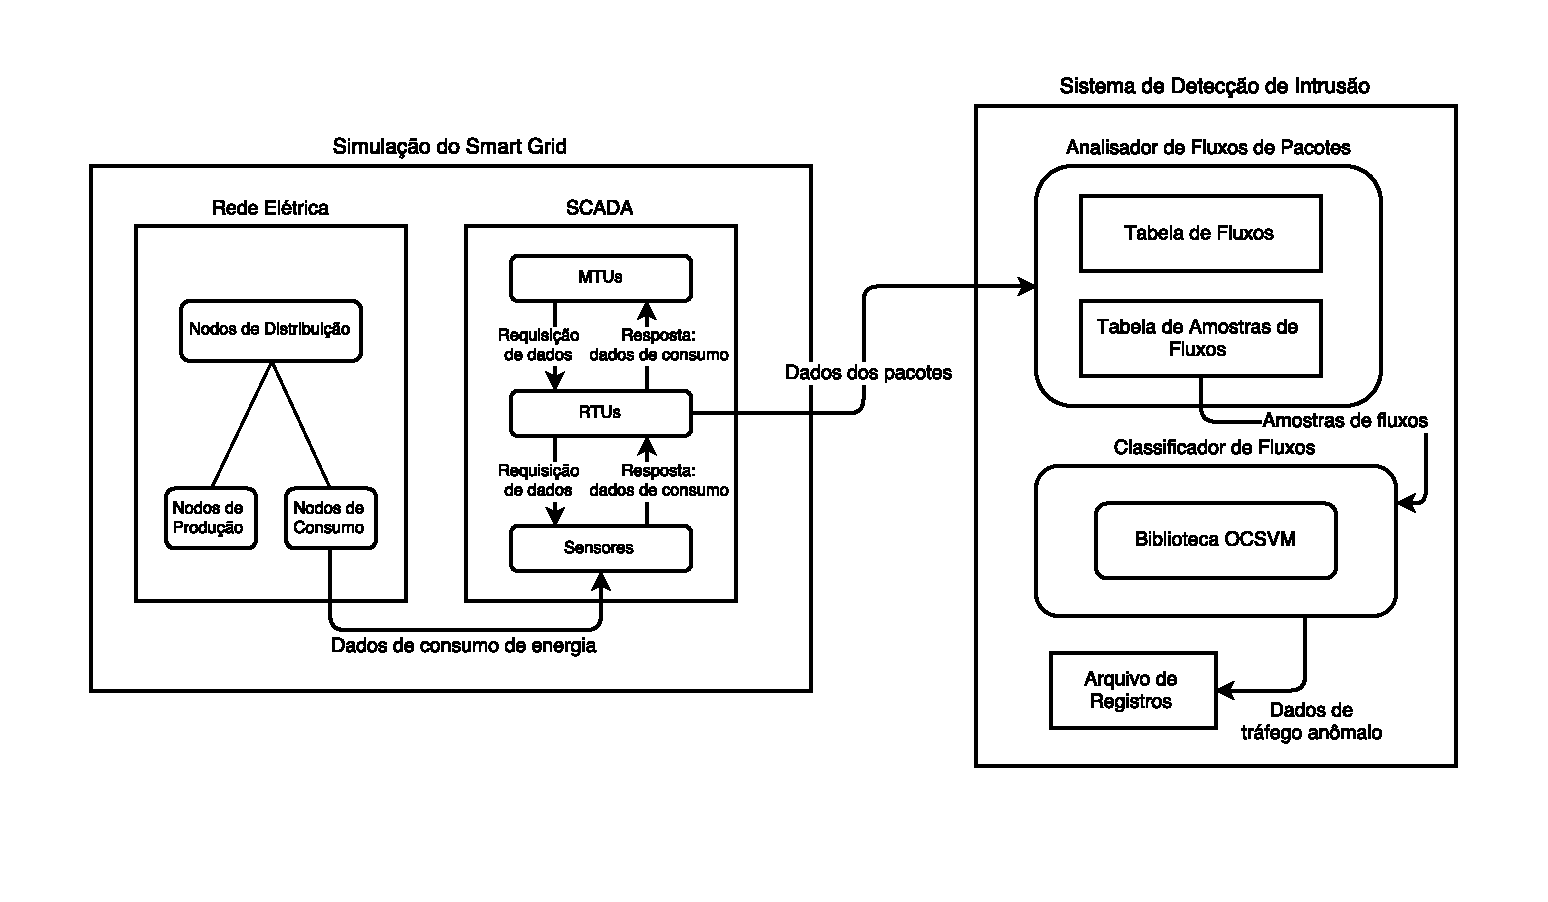
\includegraphics[width=34em]{sdi_diagram}
   \end{center}
   \legend{Fonte: Autor}
   \label{sdi_diagram}
\end{figure}

A modelagem do componente RTU no IDS é mostrada na Figura \ref{modelrtu}. Todos os pacotes de dados enviados pelos sensores para as RTUs são analisados, e as seguintes informações são recuperadas do pacote:
\begin{itemize}
\item{Origem}: Identificador do sensor que enviou o pacote para a RTU.
\item{Destino}: Identificador da RTU que recebeu o pacote.
\item{Tamanho}: Tamanho do pacote.
\item{\emph{Timestamp}}: Horário da chegada do pacote ao destino.
\end{itemize}
As informações são enviadas por um socket de rede para um servidor que implementa o Analisador de Fluxos e o Classificador de Fluxos.

\begin{figure}[h]
   \caption{Modelagem do componente RTU no IDS}
   \begin{center}
       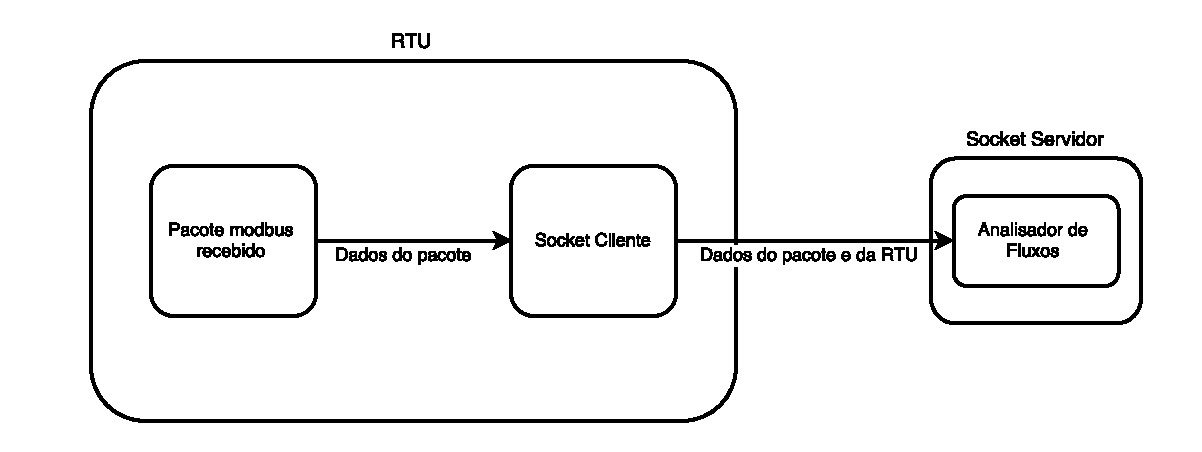
\includegraphics[width=34em]{modelrtu}
   \end{center}
   \legend{Fonte: Autor}
   \label{modelrtu}
\end{figure}

O servidor, que recebe as mensagens enviadas através do socket de rede, implementa os módulos que realizam a análise e a classificação dos dados. As mensagens recebidas pelo servidor, contendo informações sobre os pacotes, inicialmente são analisadas pelo Analisador de Fluxos, que fará a síntese dos dados que serão utilizados na classificação. O analisador recebe cada mensagem com informações de um pacote que chega ao módulo, e o insere na em duas tabelas, uma tabela de fluxos e uma tabela de amostras. Enquanto a tabela de fluxos armazena os valores computados dos atributos dos fluxos até o fim da execução, a tabela de amostras armazena amostras dos atributos dos fluxos durante um determinado período de tempo, que serão utilizadas na classificação, e depois tem seus registros deletados para o armazenamento de novas amostras. A Figura \ref{modelanalyser} apresenta a modelagem do componente Analisador de Fluxos.

Cada par de sensor de origem com RTU de destino representa um fluxo da aplicação SCADA, e os identificadores de origem e destino do pacote são utilizados para rotular cada fluxo e armazená-lo nas tabelas. Para cada fluxo identificado, os seguintes atributos são armazenados:
\begin{itemize}
\item{Quantidade de Pacotes}: Quantidade de pacotes registrados para um determinado fluxo durante toda a execução.
\item{Tamanho Médio dos Pacotes}: Tamanho médio dos pacotes de um fluxo.  
\item{Tempo Médio de Chegada Entre Pacotes}: Tempo médio entre a chegada ao destino de dois pacotes consecutivos em um mesmo fluxo.
\item{Tamanho Mínimo de Pacote}: Tamanho do maior pacote registrado em um fluxo.
\item{Tamanho Máximo de Pacote}: Tamanho do menor pacote pertencente a um fluxo.
\item{\emph{Timestamp}}: Horário de chegada ao destino do último pacote registrado no fluxo.
\end{itemize}
A cada pacote que chega, os valores de origem e destino são concatenados e utilizados como chave do registro na tabela. Caso o fluxo já exista na tabela, as informações sobre o pacote são computadas ao fluxo existente. Caso o fluxo não exista na tabela, uma nova entrada é inserida, contendo as informações sobre o primeiro pacote registrado para aquele fluxo.

As amostras armazenadas na tabela de amostras representam o comportamento de cada um dos fluxos durante um intervalo de tempo. A cada intervalo de tempo determinado, os atributos de todas as amostras são armazenados em um arquivo, e então a tabela é esvaziada de todos os dados para que as amostras do próximo intervalo de tempo sejam armazenadas.

\begin{figure}[h]
   \caption{Modelagem do componente Analisador de Fluxos no IDS}
   \begin{center}
       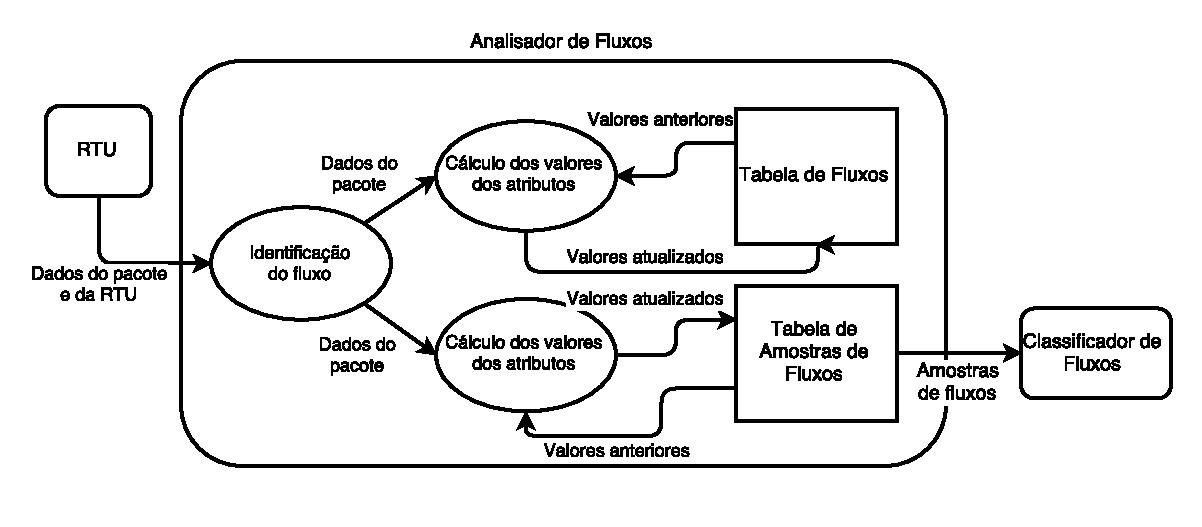
\includegraphics[width=34em]{modelanalyser}
   \end{center}
   \legend{Fonte: Autor}
   \label{modelanalyser}
\end{figure}

A modelagem do componente Classificador de Fluxos é apresentada na Figura \ref{modelclassifier}. A cada intervalo de tempo de amostragem, as amostras de fluxos são obtidas pelo classificador, e utilizadas para treinamento ou classificação. O classificador utiliza as funções da biblioteca que implementa o algoritmo OCSVM para escalar os valores das amostras recebidas e treinar o algoritmo. Quando o treinamento é encerrado, as amostras recebidas passam a ser escaladas e classificadas de acordo com o treinamento, identificando se os valores dos atributos de cada amostra pertencem ou não à classe de tráfego normal. O algoritmo é treinando e classificado utilizando os seguintes atributos para cada amostra de fluxo: 
\begin{itemize}
\item{Quantidade de Pacotes/Intervalo de Tempo}: Número de pacotes registrados para o fluxo durante o período de tempo da amostra.
\item{Tamanho Médio dos Pacotes}: Tamanho médio dos pacotes do fluxo durante o período de tempo da amostra.
\item{Tempo Médio de Chegada Entre Pacotes}: Tempo médio de chegada entre dois pacotes consecutivos ao destino durante o tempo da amostra.
\item{Tamanho Mínimo de Pacote}: Menor pacote encontrado no fluxo durante o tempo da amostra.
\item{Tamanho Máximo de Pacote}: Maior pacote encontrado no fluxo durante o tempo da amostra.
\end{itemize}
Quando uma amostra de fluxo é identificada como anômala, ela é armazenada em um arquivo de registros, que documenta todas as incidencias de tráfego anormal com as seguintes informações:
\begin{itemize}
\item{Origem}: Dispositivo do qual se origina o fluxo de rede caracterizado como tráfego anômalo.
\item{Destino}: Dispositivo que recebe os pacotes do fluxo de rede identificado como anômalo.
\item{\emph{Timestamp}}: Horário em que foi identificada a anomalia na amostra do fluxo de rede.
\item{Dados}: Valores dos atributos usados para a classificação da amostra que foi identificada como tráfego anômalo.
\end{itemize}
O arquivo de registros pode ser enviado à empresa de serviçoes públicos responsável pela manutenção do sistema SCADA, para que sejam tomadas medidas preventivas em relação à identificação de tráfego anômalo na rede ou para a condução de estudos e pesquisas sobre o tráfego do sistema.

\begin{figure}[h]
   \caption{Modelagem do componente Classificador de Fluxos no IDS}
   \begin{center}
       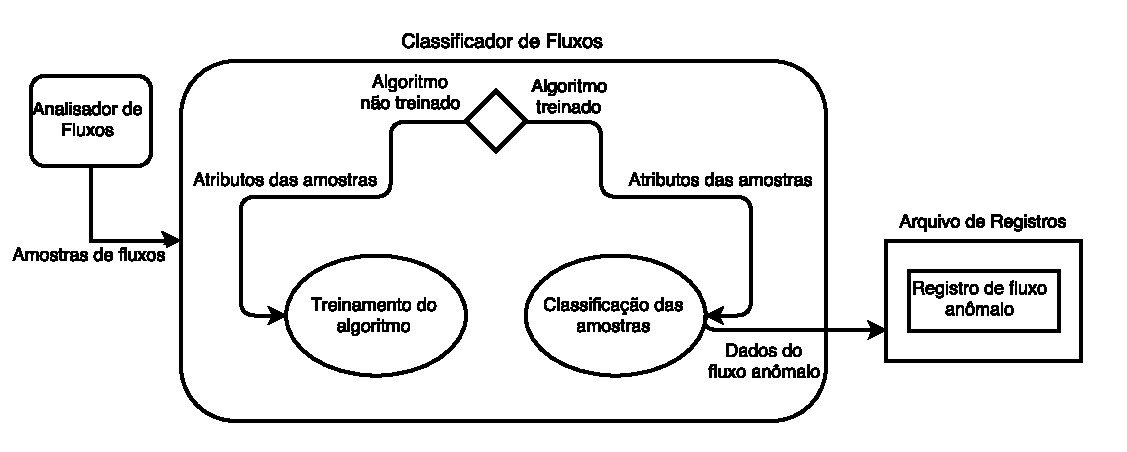
\includegraphics[width=34em]{modelclassifier}
   \end{center}
   \legend{Fonte: Autor}
   \label{modelclassifier}
\end{figure}

\begin{figure}[h]
   \caption{Diagrama de Classes do IDS Proposto}
   \begin{center}
       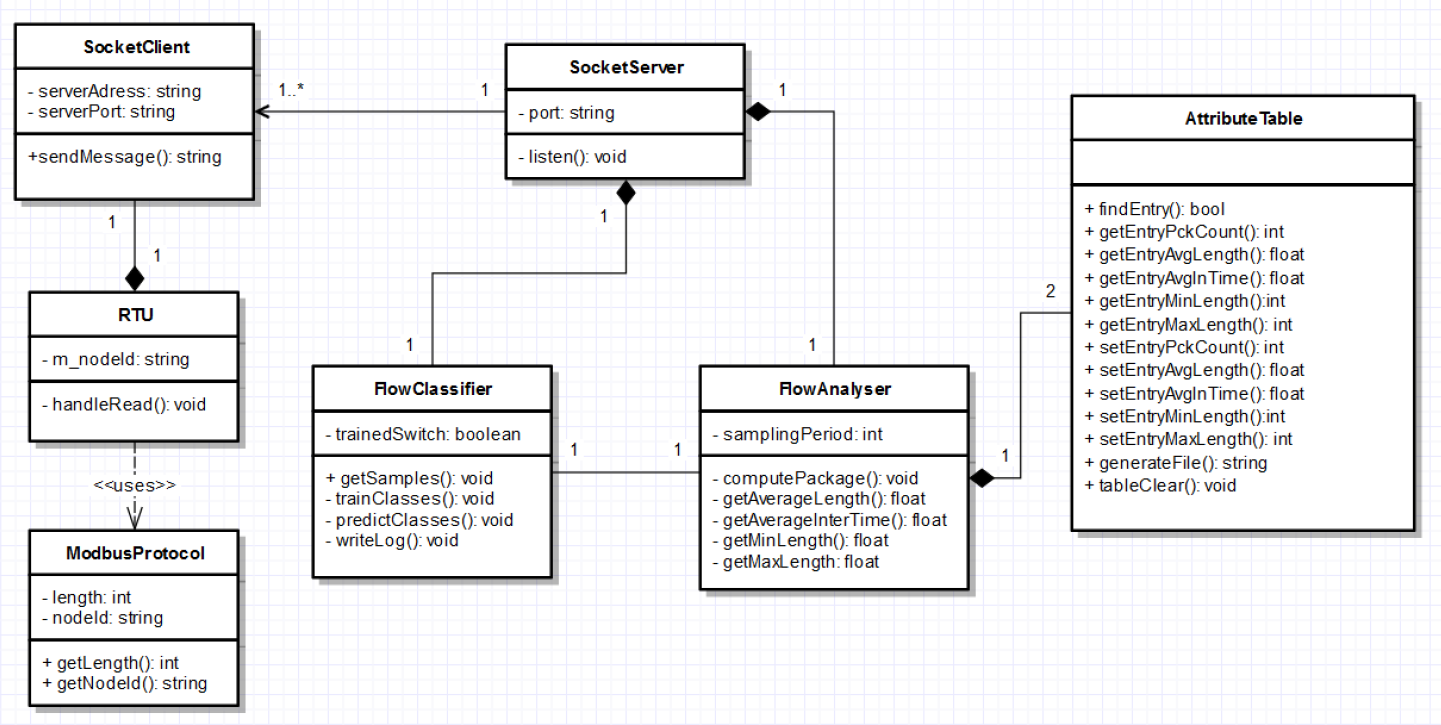
\includegraphics[width=36em]{classdiagram}
   \end{center}
   \legend{Fonte: Autor}
   \label{classdiagram}
\end{figure}

A Figura \ref{classdiagram} apresenta o diagrama de classes da estrutura do IDS. As RTUs são implementadas pela classe RTU, que gerencia os pacotes de rede enviados pelos sensores para as RTUs através da classe \emph{handleRead}. Os métodos \emph{getNodeId()} e \emph{getLength()}, da classe \emph{ModbusProtocol}, são utilizados para obter os atributos desejados do pacote, que então são concatenados em uma mensagem, juntamente com o atributo \emph{m\_NodeId} na RTU. A classe \emph{SocketClient} define um cliente que envia a mensagem, utilizando o método \emph{sendMessage()}, para um servidor, definido pela classe \emph{SocketServer}. O servidor executa o método listen() em um laço para receber mensagens, e o método \emph{computePackage()}, da classe \emph{FlowAnalyser}, é executado sobre cada mensagem que chega.

\begin{figure}[h]
   \caption{Diagrama de Sequência do IDS Proposto}
   \begin{center}
       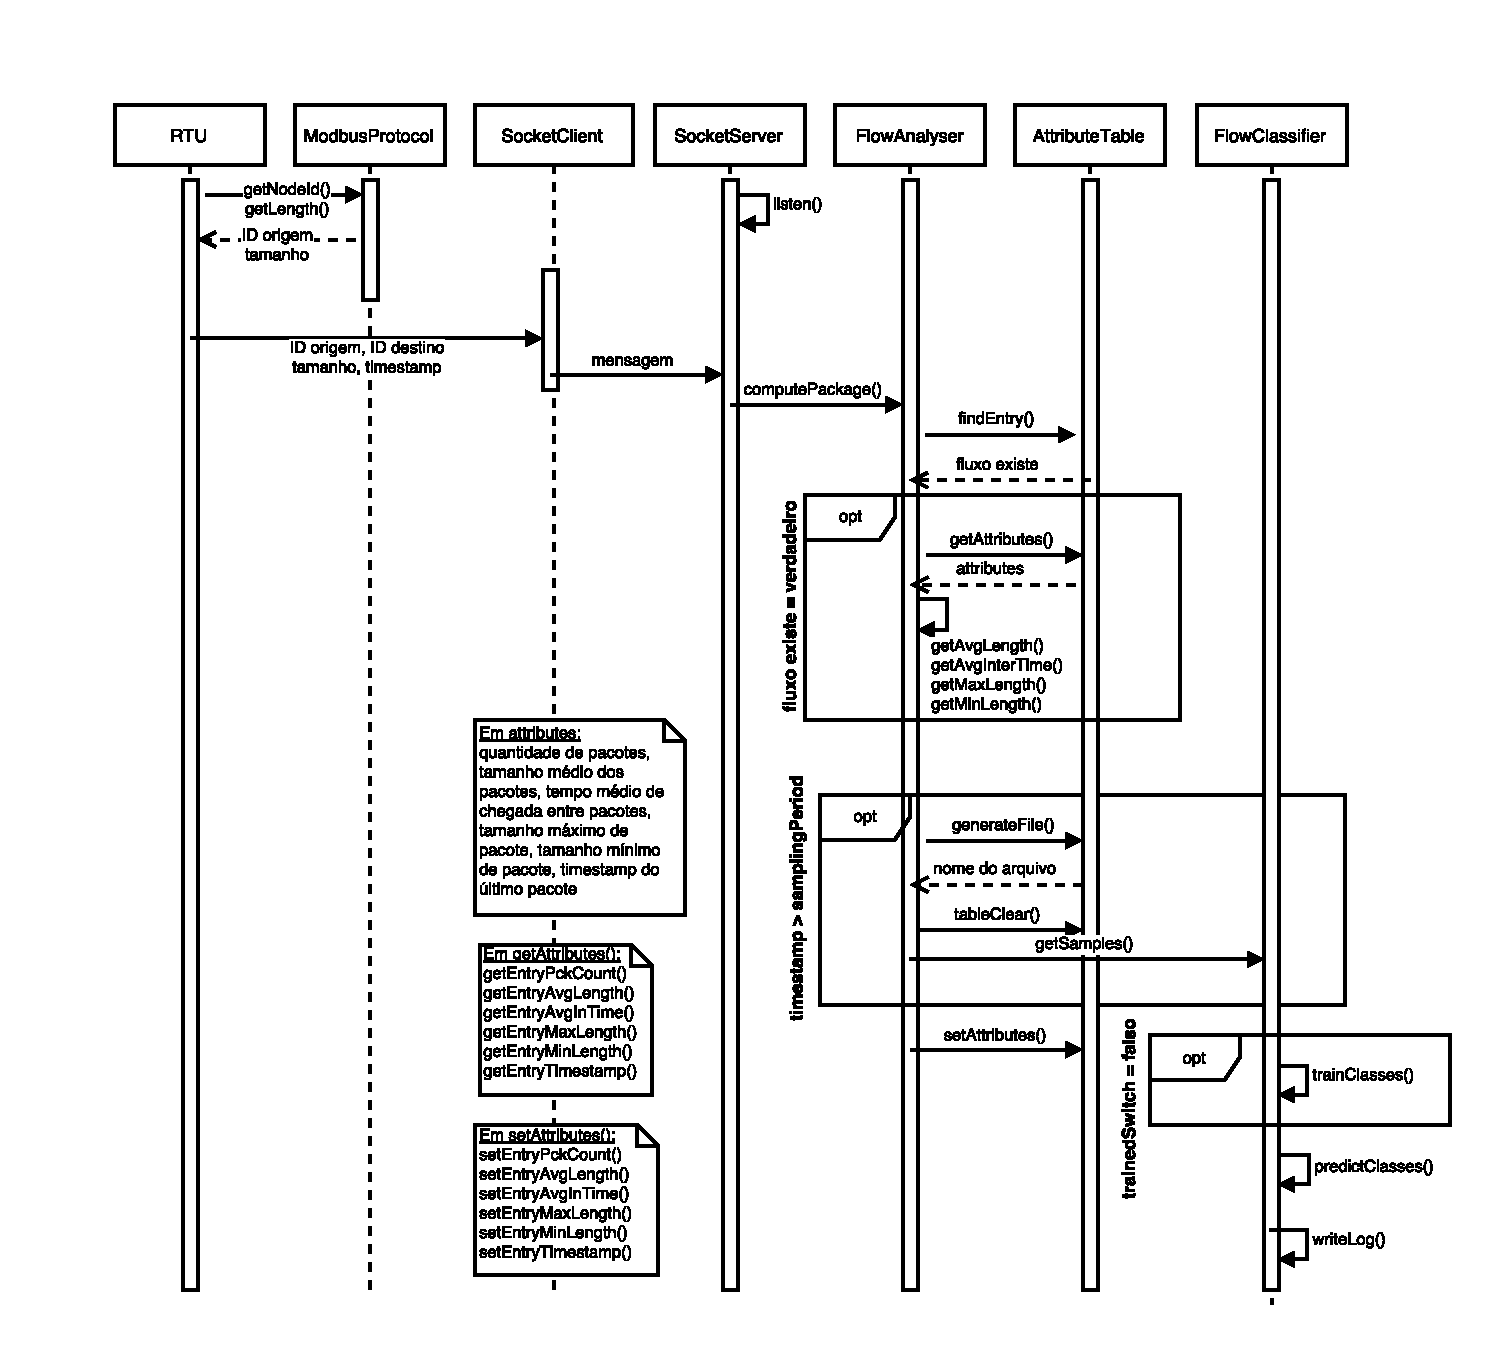
\includegraphics[width=36em]{sequencediagram}
   \end{center}
   \legend{Fonte: Autor}
   \label{sequencediagram}
\end{figure}

Na classe \emph{FlowAnalyser}, o atributo Tamanho Médio dos Pacotes de um fluxo é calculado pelo método \emph{getAveragePckSize}, utilizando a média aritmética dos tamanhos de todos os pacotes computados para aquele fluxo. O atributo Tempo Médio de Chegada Entre Pacotes é calculado pelo método \emph{getAverageInterTime}, através da média aritmética do intervalo de tempo entre a chegada de cada par de pacotes consecutivos registrados no fluxo. Os atributos Tamanho Máximo de Pacote e Tamanho Mínimo de Pacote são obtidos pelos métodos \emph{getMaxLength} e \emph{getMinLength}, respectivamente. O atributo \emph{samplingPeriod} é utilizado para definir o intervalo de tempo em que as amostras de fluxos são armazenadas, antes de serem enviadas para classificação.

As tabelas de fluxos e de amostras são definidas pela classe AttributeTable, que implementa métodos para determinar se um fluxo já existe, obter os valores dos atributos de um fluxo e inserir valores nos atributos de um fluxo. Os métodos \emph{generateFile()} e \emph{tableClear()} são utilizados para escrever os valores armazenados em um arquivo e para excluir os valores armazenados na tabela. A cada período de tempo definido em \emph{samplingPeriod}, as amostras da tabela são escritas em um arquivo e a tabela é esvaziada. O método \emph{getSamples}, da classe \emph{FlowClassifier}, obtém o arquivo de amostras gerado para classificação.

A classe \emph{FlowClassifier} implementa o método \emph{trainClasses()} para  treinar o algoritmo OCSVM, e o método \emph{predictClasses} para classificar as amostras utilizando o algoritmo treinado. Ambos os métodos escalam os valores dos atributos das amostras antes de computá-los. O atributo trainedSwitch indica se o algoritmo já está treinado ou não. O método \emph{writeLog()} é utilizado para escrever o registro dos fluxos classificados como anômalos em um arquivo. Na Figura \ref{sequencediagram}, é ilustrado o diagrama de sequência do IDS, apresentado as interações entre os métodos e os componentes do sistema.

\chapter{Implementação e Análise de Resultados}
O IDS proposto no capítulo anterior visa utilizar dados do tráfego normal de uma simulação de smart grid, obtidos a partir das RTUs, para gerar um modelo de classificação capaz de identificar tráfego anômalo. A fim de realizar a análise e avaliação desse IDS, foi implementado um protótipo para a classificação do tráfego da ferramenta ASTORIA utilizando o algoritmo OCSVM. Neste capítulo, será descrita a implementação e a avaliação do protótipo, com o objetivo de definir se o algoritmo utilizado e o modelo proposto são adequados para a identificação de anomalias em uma simulação de smart grid.

A Seção \ref{prototype} apresenta a implementação do protótipo e as ferramentas utilizadas. Na Seção \ref{sectionexp}, são descritos os experimentos executados para a avaliação do protótipo. Por fim, a Seção \ref{sectionresults} analisa os resultados obtidos nos experimentos.

\section{Implementação do Protótipo}
\label{prototype}
Para avaliar o IDS apresentado neste trabalho, foi realizada a implementação de um protótipo do sistema. O objetivo da implementação do protótipo é utilizá-lo na execução de experimentos, utilizando dados gerados a partir da simulação de um ambiente smart grid, e mensurar sua capacidade de diferenciar cenários de tráfego normal de cenários com ocorrência de ataques. 

A implementação utilizou o framework ASTORIA para a simulação do ambiente smart grid e para a geração de cenários de ataques cibernéticos, e a LIBSVM foi utilizada para a classificação dos dados de tráfego. Um cliente e o servidor UDP foram utilizados para o envio das mensagens contendo informações dos pacotes que chegam às RTUs, utilizando a biblioteca \emph{\\sys\\socket.h} e a linguagem c++. As mensagens enviadas pelo \emph{socket} são compostas por uma \emph{string} com os dados do pacote: origem, destino, tamanho e \emph{timestamp}. Os módulos do IDS também foram implementados utilizando classes da linguagem c++.

A tabela de amostras de fluxos foi implementada utilizando um mapeamento, através da biblioteca \emph{map.h} do c++, de uma chave do tipo \emph{string}, caracterizada pelos identificadores dos nodos pertencentes a cada fluxo, com um vetor de \emph{floats}, contendo os atributos armazenados para cada fluxo. Dessa forma, é possível encontrar e acessar diretamente todos os registros da tabela através da chave. O vetor de atributos armazena os seguintes valores: quantidade de pacotes, tamanho médio do pacote, tempo médio entre a chegada de pacotes, tamanho máximo de pacote, tamanho mínimo de pacote e \emph{timestamp} do último pacote recebido. Ao fim de cada período de amostragem, os dados da tabela são registrados em um arquivo de texto, e então a tabela é esvaziada para armazenar as novas amostras.

Os arquivos de texto gerados com as amostras de cada período de tempo armazenam as instâncias no seguinte formato: \emph{1 1:quantidade de pacotes 2:tamanho médio dos pacotes 3:tamanho mínimo de pacote 4:tamanho máximo de pacote 5:tempo médio entre chegada de pacotes}. Este formato é utilizado nos arquivos de entrada para os \emph{scripts} de escala, treinamento e classificação com o OCSVM utilizando a LIBSVM. Primeiramente, os arquivos são utilizados como entrada para o \emph{script svm-scale}, que produz como saída um arquivo com os dados escalados. Os dados do conjunto de treinamento são escalados para o intervalo padrão, $[-1,1]$. Os dados dos conjuntos de classificação são escalados utilizando os mesmos parâmetros de escala obtidos para o conjunto de treinamento. O treinamento do algoritmo é realizado pelo \emph{script svm-train}, que utiliza o arquivo contendo o conjunto de entrada e gera como saída um arquivo contendo o modelo de classificação. A classificação das amostras a cada período de amostragem é realizada pelo \emph{script svm-predic}, que recebe como entradas o arquivo contendo o modelo de classificação e o arquivo contendo as amostras para classificação, e produz como saída um arquivo indicando a classe à qual cada amostra pertence.

Quando uma amostra é classificada como não pertencente à classe de tráfego normal, ela é armazenada em um arquivo de registros, contendo as seguintes informações: Identificador do dispositivo de origem, identificador do despositivo de destino, atributos do fluxo e \emph{timestamp} da amostra.

\section{Execução dos Experimentos}
\label{sectionexp}
Os experimentos para avaliação do funcionamento do IDS previamente definido foram realizados através de simulações, utilizando a ferramenta ASTORIA, de diferentes cenários de um ambiente smart grid. Os dados de tráfego, gerados durante as simulações, são obtidos pelo protótipo implementado do IDS, e então utilizados como entrada para os processos de análise e classificação. Os experimentos utilizaram cenários de tráfego anômalo na simulação para testar a capacidade do IDS de identificar fluxos anormais.

Para a realização dos experimentos, foi definida uma topologia para a simulação, que representa a interação entre os componentes da rede no cenário sendo simulado. Outras características da simulação, como o intervalo de tempo entre as requisições de dados das RTUs e MTUs e a duração da simulação, também foram definidos. Em seguida, foram definidos os cenários que originam tráfego anômalo na simulação.

Na Seção \ref{subtopo}, são descritas a topologia e as configurações utilizadas na ferramenta ASTORIA para a simulação do cenário do smart grid. A Seção \ref{subattacks} descreve os recursos utilizados para gerar os cenários de tráfego anômalo, utilizados para testar o funcionamento do IDS.

\subsection{Topologia e Configuração das Simulações}
\label{subtopo}
A topologia utilizada nas simulações do smart grid com o ASTORIA é ilustrada na Figura \ref{figtopology}, e é composta por 1 MTU, 14 RTUs e 168 sensores.
\begin{itemize}
\item{MTU}: A MTU envia requisições às RTUs, que enviam respostas contendo dados sobre os valores de energia medidos pelos sensores naquela região. Todas as RTUs da simulação estão conectadas à MTU. Como a MTU é o único componente do sistema SCADA na simulação que não tem um correspondente na rede de energia, ela existe apenas na rede de comunicação.
\item{RTUs}: As RTUs enviam requisições aos sensores, que respondem enviando os dados sobre consumo de energia coletados por eles. Cada RTU possui 12 sensores conectados a ela e está conectada à MTU. Para toda RTU na simulação, existe um nodo de distribuição de energia na rede elétrica associado a ela.
\item{Sensores}: Cada um dos sensores na simulação está conectado à uma RTU, e possui um nodo de consumo de energia associado a ele na rede elétrica. Quando uma requisição da RTU chega ao sensor, ele responde enviando os dados medidos de consumo de energia no seu respectivo nodo.
\end{itemize}

\begin{figure}[h]
   \caption{Topologia utilizada nos experimentos}
   \begin{center}
       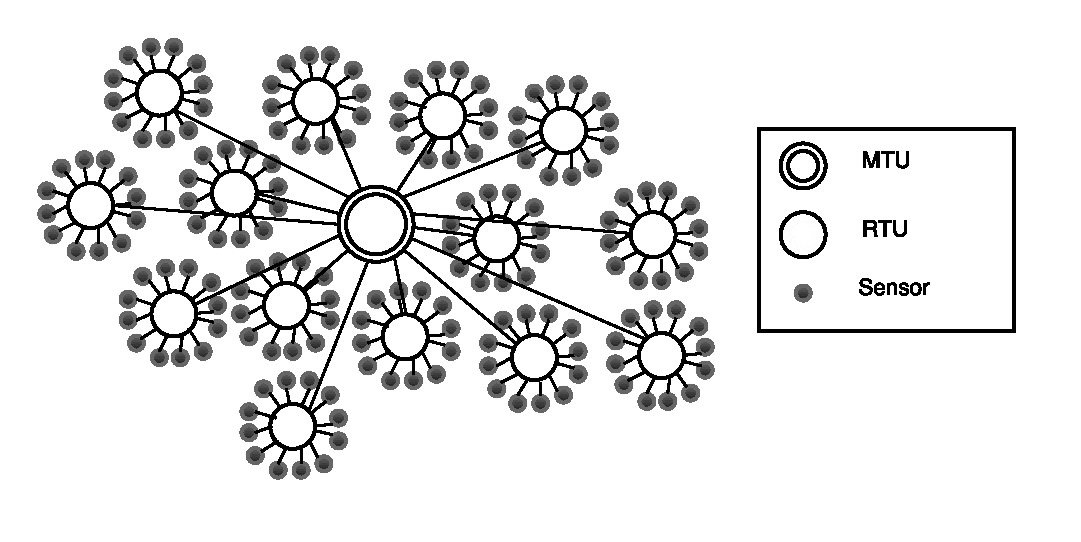
\includegraphics[width=30em]{topologia}
   \end{center}
   \legend{Fonte: Autor}
   \label{figtopology}
\end{figure}


Na configuração das simulações, o tempo total de execução foi definido em 1800 segundos e o passo de execução foi definido em 2 segundos. O passo de execução define que, a cada 2 segundos, todas as RTUs enviarão requisições de dados para todos os seus respectivos sensores, e a MTU enviará requisições de dados para todas as RTUs. Para a realização dos experimentos, foram utilizados dois modelos de simulação. O primeiro modelo de simulação utiliza o tráfego puro gerado pela configuração que foi definida. Nesse modelo, as requisições são enviadas a cada intervalo de 2 segundos, sem variações, e as amostras de tráfego obtidas tem valores constantes. Ao calcular os atributos dos fluxos do tráfego desse modelo de simulação, os valores obtidos tendem a convergir, gerando amostras uniformes, com variações muito pequenas. No segundo modelo de simulação, atrasos aleatórios são introduzidos ao intervalo de tempo entre as requisições enviadas por algumas RTUs, causando variações nos intervalos de envio das requisições. Cada requisição enviada por uma RTU tem uma chance de 25\% de sofrer um atraso aleatório de 100, 200, 300 ou 400 milissegundos. Esse modelo gera amostras de tráfego com maior variedade, e os valores calculados para os atributos dos fluxos apresentam resultados com maior diversidade de valores.

As informações de tráfego gerado por cada um dos modelos de simulação foram utilizadas nos experimentos para o treinamento do IDS, a fim de gerar um modelo de classificação capaz de reconhecer o tráfego normal da simulação. Após o treinamento  utilizando tráfego normal da simulação, os dados de tráfego gerados pelas simulações com anomalias inseridas foram analisados e classificados pelo IDS, para testar a capacidade da ferramenta de reconhecer os fluxos de tráfego anômalos.

\subsection{Introdução de Tráfego Anômalo}
\label{subattacks} 
O primeiro recurso utilizado para a geração de anomalias no cenário da simulação foi o ataque DoS fornecido pelo framework ASTORIA. Dois perfis de ataque foram utilizados no experimento, ambos os ataques com as RTUs 4 e 9 sendo atacadas por um de seus respectivos sensores. O primeiro perfil define um ataque de alta potência, com o intervalo de envio de pacotes variando entre 2 e 50 milissegundos, o que gera entre 20 e 500 pacotes por segundo sendo enviados a cada uma das RTUs sob ataque, em contraste à média de 0,5 pacote por segundo, característica do tráfego normal da simulação. No segundo perfil, o ataque realizado é de baixa potência, e o intervalo de envio dos pacotes varia entre 200 e 500 milissegundos, enviando entre 2 e 5 pacotes por segundo para as RTUs sob ataque.

O tamanho dos pacotes enviados pelos componentes não pode ser manipulado de maneira simples em uma simulação, pois ele é definido pela carga de dados enviada pelos sensores. Dessa forma, afim de obter dados de tráfego com anomalias no tamanho dos pacotes para os experimentos, foram geradas cargas de dados com alteração nos tamanhos dos pacotes obtidos. Os conjuntos de dados gerados são semelhantes aos dados obtidos de uma simulação normal, mas com variações inseridas nos valores obtidos para o tamanho dos pacotes em alguns fluxos. Os valores anômalos inseridos incluíram pacotes com 80\%, 120\%, 200\% e 400\% do tamanho original.

As anomalias geradas foram utilizadas em experimentos nos dois modelos de simulação, o modelo de tráfego uniforme e o modelo de tráfego com variações. Assim, os seguintes experimentos foram executados, cada um com 10 repetições:
\begin{itemize}
\item{}Simulação com modelo de tráfego uniforme com o perfil de ataque DoS de alta potência
\item{}Simulação com modelo de tráfego com variações com o perfil de ataque DoS de alta potência
\item{}Simulação com modelo de tráfego uniforme com o perfil de ataque DoS de baixa potência
\item{}Simulação com modelo de tráfego com variações com o perfil de ataque DoS de baixa potência
\item{}Simulação com modelo de tráfego uniforme com a carga de dados contendo anomalias no tamanho dos pacotes
\item{}Simulação com modelo de tráfego com variações com a carga de dados contendo anomalias no tamanho dos pacotes
\end{itemize}

\section{Análise dos Resultados}
\label{sectionresults}

Para a avaliação dos resultados obtidos nos experimentos, foram utilizadas as métricas Taxa de Verdadeiros Positivos (TVP),  Taxa de Falsos Positivos (TFP), Taxa de Verdadeiros Negativos(TVN) e Taxa de Falsos Negativos (TFN), amplamente utilizados na avaliação de sistemas de classificação [nguyen].
\begin{itemize}
\item{Taxa de Verdadeiros Positivos}: Porcentagem de amostras de tráfego normal, classificadas corretamente como pertencentes à classe de tráfego normal, dada por $TVP = VP / (VP + FN)$.
\item{Taxa de Verdadeiros Negativos}: Porcentagem de amostras de tráfego anômalo, classificadas corretamente como não pertencentes à classe de tráfego normal, calculada a partir de $TVN = VN / (VN + FP)$.
\item{Taxa de Falsos Positivos}: Porcentagem de amostras de tráfego anômalo, classificadas incorretamente como pertencentes à classe de tráfego normal, calculada por $TFP = 1 - TVN$.
\item{Taxa de Falsos Negativos}: Porcentagem de amostras de tráfego normal classificadas incorretamente como não pertencentes à classe de tráfego normal, obtida com $TFN = 1 - TVP$.
\item{Acurácia}: medida que representa a porcentagem de amostras classificadas corretamente em relação à quantidade total de amostras, calculada pela expressão $ACC = (VP + VN) / (VP + VN + FP + FN)$.
\end{itemize}

\begin{figure}[h]
   \caption{Resultados dos experimentos com um ataque DoS de alta potência}
   \begin{center}
       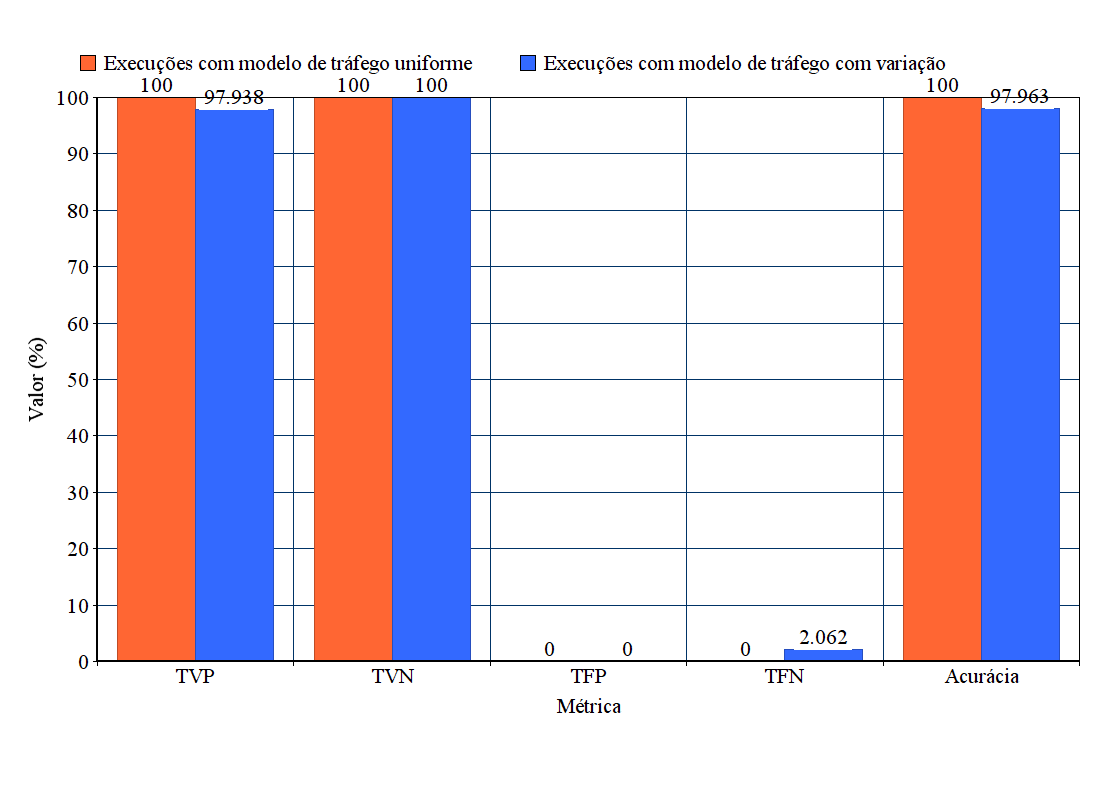
\includegraphics[width=30em]{chartdos1}
   \end{center}
   \legend{Fonte: Autor}
   \label{chartdos1}
\end{figure}

A Figura \ref{chartdos1} apresenta os resultados obtidos na classificação do tráfego da simulação durante a ocorrência de um ataque DoS de alta potência. Primeiramente, é possível observar que, nos experimentos que utilizaram a simulação com modelo de tráfego uniforme, o IDS foi capaz de classificar corretamente todas as amostras, atingindo uma acurácia de 100\%. Já nos experimentos que utilizaram a simulação com modelo de tráfego com variações, apesar do IDS ter identificado corretamente todas as amostras de tráfego anômalo, uma parcela das amostras de fluxos normais foram classificadas como anômalas, gerando uma TFN de 2,062\%. Podemos atribuir esses resultados ao modelo de classificação que é gerado pelo IDS. Quando utilzamos o modelo de tráfego uniforme, o tráfego se mantém constante ao longo da execução, gerando amostras de tráfego que possuem valores de atributos iguais ou com variações muito pequenas. Quando essas amostras são utilizadas no treinamento do algoritmo, o modelo gerado para solucionar a classificação é muito simples, pois amostras de tráfego normal sempre serão iguais às amostras utilizadas no treinamento, e qualquer amostra com uma pequena variação é caracterizada como anômala. Quando o modelo de tráfego com variações é utilizado, as amostras de tráfego utilizadas para o treinamento do algoritmo sofrem variações aleatórias, o que torna o problema da classificação mais complexo. O classificador de classe única não é capaz de incorporar toda a diversidade de dados do conjunto de treinamento ao modelo de classificação. Assim, algumas amostras com variações, provenientes de tráfego normal, são consideradas fora da classe descrita pelo modelo, e classificadas como anômalas. Ainda assim, o classificador obteve acurácia de 97,963\% na classificação do tráfego nesse cenário.

\begin{figure}[h]
   \caption{Resultados dos experimentos com um ataque DoS de baixa potência}
   \begin{center}
       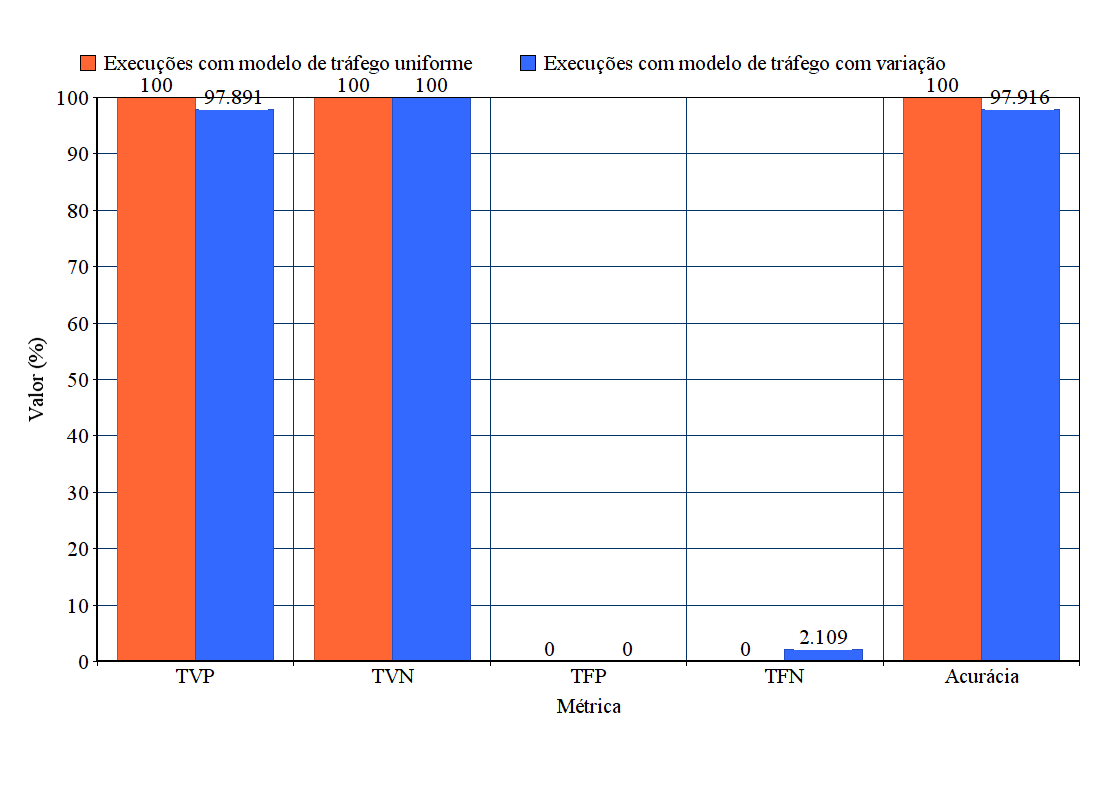
\includegraphics[width=30em]{chartdos2}
   \end{center}
   \legend{Fonte: Autor}
   \label{chartdos2}
\end{figure}

Os resultados obtidos para a classificação do tráfego durante um ataque DoS de baixa potência são mostrados na Figura \ref{chartdos2}. Os resultados obtidos para esse cenário são semelhantes aos resultados obtidos nos cenários com o ataque DoS de alta potência. Nas execuções com a simulação de modelo uniforme de tráfego, o IDS também classificou corretamente todas as amostras, com 100\% de acurácia. Nas execuções com a simulação de modelo de tráfego com variações, as amostras de fluxos provenientes dos ataques também foram 100\% classificadas como anômalas, mas com uma TFN de 2,109\%, obtendo 97,916\% de acurácia. Da mesma forma que nos experimentos com o ataque de alta potência, o modelo de classificação gerado a partir da simulação de tráfego com variações não compreendeu toda a diversidade de dados descrita pelas amostras de tráfego. Desse modo, apesar das anomalias geradas serem mais próximas do tráfego normal, o classificador as excluiu as amostras anômalas da classe normal da mesma forma que excluiu parte das amostras normais que possuíam variações.

\begin{figure}[h]
   \caption{Resultados dos experimentos com inserção de anomalias no tamanho dos pacotes}
   \begin{center}
       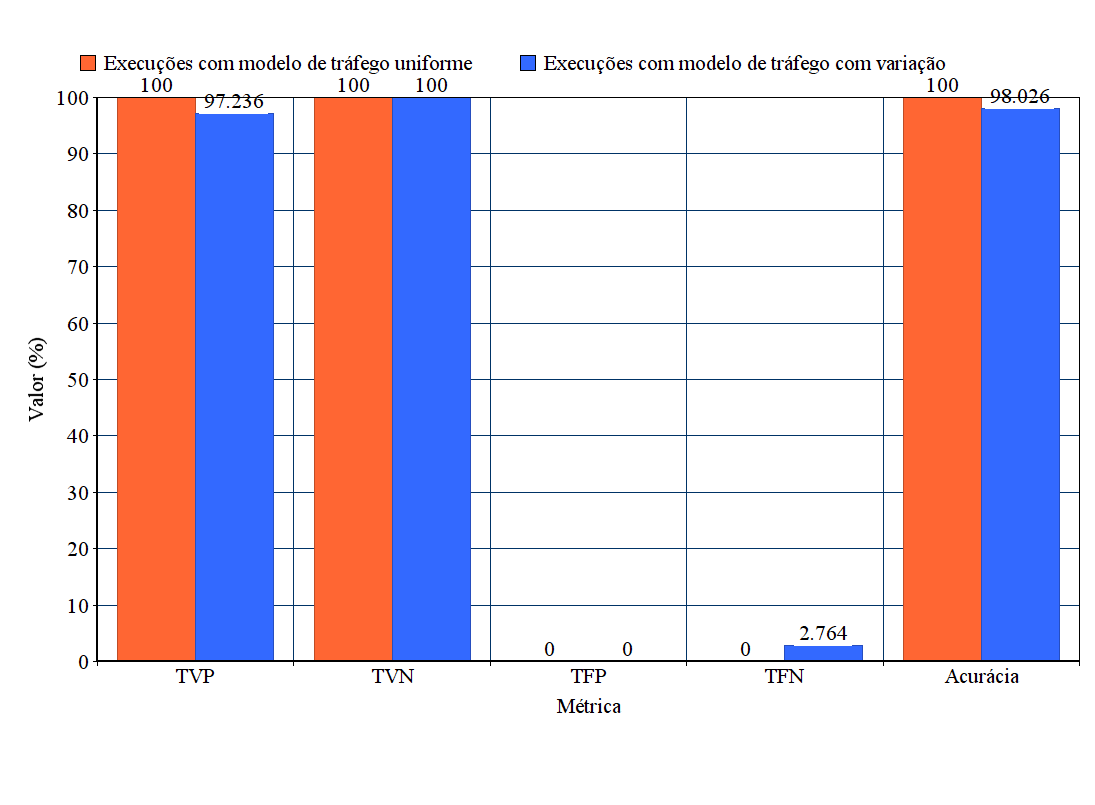
\includegraphics[width=30em]{chartsize}
   \end{center}
   \legend{Fonte: Autor}
   \label{chartsize}
\end{figure}

Por fim, a Figura \ref{chartsize} apresenta os resultados obtidos para a classificação do tráfego utilizando cargas de dados com anomalias no tamanho dos pacotes. Os resultados seguiram o mesmo comportamento dos experimentos com os cenários de ataques DoS. As execuções utilizando a simulação com o modelo de tráfego uniforme obtiveram acurácia de 100\% na classificação. As execuções utilizando a simulação com modelo de tráfego com variação identificaram todas as amostras anômalas corretamente, porém com uma TFN de 2,764\%, atingindo 98,026\% de acurácia.

A primeira consideração que pode ser feita sobre os resultados obtidos é que o classificador obtém resultados mais precisos para a classificação de tráfegos mais estáveis, com maior uniformidade nos dados e poucas variações. Quando pequenas variações são inseridas no tráfego, o modelo de classificação gerado passa a não assimilar toda a diversidade de dados presente no conjunto de treinamento, e falsos negativos passam a ocorrer na classificação. Todavia, a TFP foi zero em todos os experimentos, indicando que todas as ocorrências de tráfego anômalo foram identificadas, e a acurácia superou 97\% em todas as execuções. Esses resultados apontam que IDSs baseados no algoritmo OCSVM são viáveis em estruturas de comunicação de smart grids.

Para aumentar a precisão do IDS, seria possível complementar o algoritmo de detecção de anomalias com um algoritmo SBD de reconhecimento de perfis de ataque. Dessa forma, todas as amostras de fluxo identificadas como anômalas pelo classificador poderiam ser comparadas aos perfis de ataques registrados. Esse processo poderia identificar os verdadeiros negativos através da similaridade com os perfis de ataque, e eliminar os falsos negativos. Para isso, seria necessário ter acesso a dados sobre o comportamento do tráfego da rede do smart grid durante a ocorrência de um ataque. Outra possibilidade seria utilizar na classificação um algoritmo de classificação em duas classes, como o SVM tradicional. Nesse caso, o conjunto de treinamento seria composto por uma classe positiva, representada por amostras de tráfego normal, e uma classe negativa, representada por amostras de tráfego em cenários de ataques ou anomalias. Dessa forma, pequenas variações de tráfego estariam muito mais próximas da classe positiva do que da classe negativa, diminuindo a ocorrência de falsos negativos.

\chapter{Conclusão e Trabalhos Futuros}
\section{Resumo de Contribuições}
\section{Trabalhos Futuros}

% referências
% aqui será usado o environment padrao `thebibliography'; porém, sugere-se
% seriamente o uso de BibTeX e do estilo abnt.bst (veja na página do
% UTUG)
% 
% observe também o estilo meio estranho de alguns labels; isso é
% devido ao uso do pacote `natbib', que permite fazer citações de
% autores, ano, e diversas combinações desses

\bibliographystyle{abntex2-alf}
\bibliography{biblio}

\end{document}
